\documentclass[twoside]{book}

% Packages required by doxygen
\usepackage{fixltx2e}
\usepackage{calc}
\usepackage{doxygen}
\usepackage[export]{adjustbox} % also loads graphicx
\usepackage{graphicx}
\usepackage[utf8]{inputenc}
\usepackage{makeidx}
\usepackage{multicol}
\usepackage{multirow}
\PassOptionsToPackage{warn}{textcomp}
\usepackage{textcomp}
\usepackage[nointegrals]{wasysym}
\usepackage[table]{xcolor}

% Font selection
\usepackage[T1]{fontenc}
\usepackage[scaled=.90]{helvet}
\usepackage{courier}
\usepackage{amssymb}
\usepackage{sectsty}
\renewcommand{\familydefault}{\sfdefault}
\allsectionsfont{%
  \fontseries{bc}\selectfont%
  \color{darkgray}%
}
\renewcommand{\DoxyLabelFont}{%
  \fontseries{bc}\selectfont%
  \color{darkgray}%
}
\newcommand{\+}{\discretionary{\mbox{\scriptsize$\hookleftarrow$}}{}{}}

% Page & text layout
\usepackage{geometry}
\geometry{%
  a4paper,%
  top=2.5cm,%
  bottom=2.5cm,%
  left=2.5cm,%
  right=2.5cm%
}
\tolerance=750
\hfuzz=15pt
\hbadness=750
\setlength{\emergencystretch}{15pt}
\setlength{\parindent}{0cm}
\setlength{\parskip}{3ex plus 2ex minus 2ex}
\makeatletter
\renewcommand{\paragraph}{%
  \@startsection{paragraph}{4}{0ex}{-1.0ex}{1.0ex}{%
    \normalfont\normalsize\bfseries\SS@parafont%
  }%
}
\renewcommand{\subparagraph}{%
  \@startsection{subparagraph}{5}{0ex}{-1.0ex}{1.0ex}{%
    \normalfont\normalsize\bfseries\SS@subparafont%
  }%
}
\makeatother

% Headers & footers
\usepackage{fancyhdr}
\pagestyle{fancyplain}
\fancyhead[LE]{\fancyplain{}{\bfseries\thepage}}
\fancyhead[CE]{\fancyplain{}{}}
\fancyhead[RE]{\fancyplain{}{\bfseries\leftmark}}
\fancyhead[LO]{\fancyplain{}{\bfseries\rightmark}}
\fancyhead[CO]{\fancyplain{}{}}
\fancyhead[RO]{\fancyplain{}{\bfseries\thepage}}
\fancyfoot[LE]{\fancyplain{}{}}
\fancyfoot[CE]{\fancyplain{}{}}
\fancyfoot[RE]{\fancyplain{}{\bfseries\scriptsize Generated by Doxygen }}
\fancyfoot[LO]{\fancyplain{}{\bfseries\scriptsize Generated by Doxygen }}
\fancyfoot[CO]{\fancyplain{}{}}
\fancyfoot[RO]{\fancyplain{}{}}
\renewcommand{\footrulewidth}{0.4pt}
\renewcommand{\chaptermark}[1]{%
  \markboth{#1}{}%
}
\renewcommand{\sectionmark}[1]{%
  \markright{\thesection\ #1}%
}

% Indices & bibliography
\usepackage{natbib}
\usepackage[titles]{tocloft}
\setcounter{tocdepth}{3}
\setcounter{secnumdepth}{5}
\makeindex

% Hyperlinks (required, but should be loaded last)
\usepackage{ifpdf}
\ifpdf
  \usepackage[pdftex,pagebackref=true]{hyperref}
\else
  \usepackage[ps2pdf,pagebackref=true]{hyperref}
\fi
\hypersetup{%
  colorlinks=true,%
  linkcolor=blue,%
  citecolor=blue,%
  unicode%
}

% Custom commands
\newcommand{\clearemptydoublepage}{%
  \newpage{\pagestyle{empty}\cleardoublepage}%
}

\usepackage{caption}
\captionsetup{labelsep=space,justification=centering,font={bf},singlelinecheck=off,skip=4pt,position=top}

%===== C O N T E N T S =====

\begin{document}

% Titlepage & ToC
\hypersetup{pageanchor=false,
             bookmarksnumbered=true,
             pdfencoding=unicode
            }
\pagenumbering{alph}
\begin{titlepage}
\vspace*{7cm}
\begin{center}%
{\Large Catch The Bus Prototype }\\
\vspace*{1cm}
{\large Generated by Doxygen 1.8.14}\\
\end{center}
\end{titlepage}
\clearemptydoublepage
\pagenumbering{roman}
\tableofcontents
\clearemptydoublepage
\pagenumbering{arabic}
\hypersetup{pageanchor=true}

%--- Begin generated contents ---
\chapter{Catch-\/the-\/\+Bus}
\label{md__r_e_a_d_m_e}
\Hypertarget{md__r_e_a_d_m_e}
Software Engineering Project for E\+E\+CS 448 \subsection*{About This Project}

Code Chefs are cooking up an isometric arcade game. We\textquotesingle{}re planning to use Unity for Android development.

\subsubsection*{Features Being Worked On}


\begin{DoxyItemize}
\item Unity Learning
\item Version Control
\item Prototype
\item Basic Art/\+Sound 
\end{DoxyItemize}
\chapter{Namespace Index}
\section{Packages}
Here are the packages with brief descriptions (if available)\+:\begin{DoxyCompactList}
\item\contentsline{section}{\mbox{\hyperlink{namespace_mega_dad}{Mega\+Dad}} }{\pageref{namespace_mega_dad}}{}
\item\contentsline{section}{\mbox{\hyperlink{namespace_super_tiled2_unity}{Super\+Tiled2\+Unity}} }{\pageref{namespace_super_tiled2_unity}}{}
\item\contentsline{section}{\mbox{\hyperlink{namespace_super_tiled2_unity_1_1_editor}{Super\+Tiled2\+Unity.\+Editor}} }{\pageref{namespace_super_tiled2_unity_1_1_editor}}{}
\item\contentsline{section}{\mbox{\hyperlink{namespace_super_tiled2_unity_1_1_editor_1_1_clipper_lib}{Super\+Tiled2\+Unity.\+Editor.\+Clipper\+Lib}} }{\pageref{namespace_super_tiled2_unity_1_1_editor_1_1_clipper_lib}}{}
\item\contentsline{section}{\mbox{\hyperlink{namespace_super_tiled2_unity_1_1_editor_1_1_geometry}{Super\+Tiled2\+Unity.\+Editor.\+Geometry}} }{\pageref{namespace_super_tiled2_unity_1_1_editor_1_1_geometry}}{}
\item\contentsline{section}{\mbox{\hyperlink{namespace_super_tiled2_unity_1_1_editor_1_1_lib_tess_dot_net}{Super\+Tiled2\+Unity.\+Editor.\+Lib\+Tess\+Dot\+Net}} }{\pageref{namespace_super_tiled2_unity_1_1_editor_1_1_lib_tess_dot_net}}{}
\item\contentsline{section}{\mbox{\hyperlink{namespace_super_tiled2_unity_1_1_editor_1_1_s_d}{Super\+Tiled2\+Unity.\+Editor.\+SD}} }{\pageref{namespace_super_tiled2_unity_1_1_editor_1_1_s_d}}{}
\item\contentsline{section}{\mbox{\hyperlink{namespace_super_tiled2_unity_1_1_editor_1_1_s_d_1_1_tools}{Super\+Tiled2\+Unity.\+Editor.\+S\+D.\+Tools}} }{\pageref{namespace_super_tiled2_unity_1_1_editor_1_1_s_d_1_1_tools}}{}
\item\contentsline{section}{\mbox{\hyperlink{namespace_super_tiled2_unity_1_1_editor_1_1_s_d_1_1_tools_1_1_algorithmia}{Super\+Tiled2\+Unity.\+Editor.\+S\+D.\+Tools.\+Algorithmia}} }{\pageref{namespace_super_tiled2_unity_1_1_editor_1_1_s_d_1_1_tools_1_1_algorithmia}}{}
\item\contentsline{section}{\mbox{\hyperlink{namespace_super_tiled2_unity_1_1_editor_1_1_s_d_1_1_tools_1_1_algorithmia_1_1_general_data_structures}{Super\+Tiled2\+Unity.\+Editor.\+S\+D.\+Tools.\+Algorithmia.\+General\+Data\+Structures}} }{\pageref{namespace_super_tiled2_unity_1_1_editor_1_1_s_d_1_1_tools_1_1_algorithmia_1_1_general_data_structures}}{}
\item\contentsline{section}{\mbox{\hyperlink{namespace_super_tiled2_unity_1_1_editor_1_1_third_party}{Super\+Tiled2\+Unity.\+Editor.\+Third\+Party}} }{\pageref{namespace_super_tiled2_unity_1_1_editor_1_1_third_party}}{}
\item\contentsline{section}{\mbox{\hyperlink{namespace_super_tiled2_unity_1_1_ionic}{Super\+Tiled2\+Unity.\+Ionic}} }{\pageref{namespace_super_tiled2_unity_1_1_ionic}}{}
\item\contentsline{section}{\mbox{\hyperlink{namespace_super_tiled2_unity_1_1_ionic_1_1_b_zip2}{Super\+Tiled2\+Unity.\+Ionic.\+B\+Zip2}} }{\pageref{namespace_super_tiled2_unity_1_1_ionic_1_1_b_zip2}}{}
\item\contentsline{section}{\mbox{\hyperlink{namespace_super_tiled2_unity_1_1_ionic_1_1_crc}{Super\+Tiled2\+Unity.\+Ionic.\+Crc}} }{\pageref{namespace_super_tiled2_unity_1_1_ionic_1_1_crc}}{}
\item\contentsline{section}{\mbox{\hyperlink{namespace_super_tiled2_unity_1_1_ionic_1_1_encoding}{Super\+Tiled2\+Unity.\+Ionic.\+Encoding}} }{\pageref{namespace_super_tiled2_unity_1_1_ionic_1_1_encoding}}{}
\item\contentsline{section}{\mbox{\hyperlink{namespace_super_tiled2_unity_1_1_ionic_1_1_zip}{Super\+Tiled2\+Unity.\+Ionic.\+Zip}} }{\pageref{namespace_super_tiled2_unity_1_1_ionic_1_1_zip}}{}
\item\contentsline{section}{\mbox{\hyperlink{namespace_super_tiled2_unity_1_1_ionic_1_1_zlib}{Super\+Tiled2\+Unity.\+Ionic.\+Zlib}} }{\pageref{namespace_super_tiled2_unity_1_1_ionic_1_1_zlib}}{}
\item\contentsline{section}{\mbox{\hyperlink{namespace_tests}{Tests}} }{\pageref{namespace_tests}}{}
\item\contentsline{section}{\mbox{\hyperlink{namespace_tests_1_1_editor}{Tests.\+Editor}} }{\pageref{namespace_tests_1_1_editor}}{}
\item\contentsline{section}{\mbox{\hyperlink{namespace_tiled2_unity}{Tiled2\+Unity}} }{\pageref{namespace_tiled2_unity}}{}
\end{DoxyCompactList}

\chapter{Hierarchical Index}
\section{Class Hierarchy}
This inheritance list is sorted roughly, but not completely, alphabetically\+:\begin{DoxyCompactList}
\item Asset\+Postprocessor\begin{DoxyCompactList}
\item \contentsline{section}{Tiled2\+Unity.\+Tiled\+Asset\+Post\+Processor}{\pageref{class_tiled2_unity_1_1_tiled_asset_post_processor}}{}
\end{DoxyCompactList}
\item Attribute\begin{DoxyCompactList}
\item \contentsline{section}{Tiled2\+Unity.\+Custom\+Tiled\+Importer\+Attribute}{\pageref{class_tiled2_unity_1_1_custom_tiled_importer_attribute}}{}
\end{DoxyCompactList}
\item Editor\begin{DoxyCompactList}
\item \contentsline{section}{Sorting\+Layer\+Exposed\+Editor}{\pageref{class_sorting_layer_exposed_editor}}{}
\item \contentsline{section}{Tiled2\+Unity.\+Sprite\+Depth\+In\+Map\+Editor}{\pageref{class_tiled2_unity_1_1_sprite_depth_in_map_editor}}{}
\end{DoxyCompactList}
\item \contentsline{section}{Tiled2\+Unity.\+I\+Custom\+Tiled\+Importer}{\pageref{interface_tiled2_unity_1_1_i_custom_tiled_importer}}{}
\item I\+Disposable\begin{DoxyCompactList}
\item \contentsline{section}{Tiled2\+Unity.\+Import\+Tiled2\+Unity}{\pageref{class_tiled2_unity_1_1_import_tiled2_unity}}{}
\item \contentsline{section}{Tiled2\+Unity.\+Logger}{\pageref{class_tiled2_unity_1_1_logger}}{}
\end{DoxyCompactList}
\item I\+Drag\+Handler\begin{DoxyCompactList}
\item \contentsline{section}{Joystick}{\pageref{class_joystick}}{}
\begin{DoxyCompactList}
\item \contentsline{section}{Fixed\+Joystick}{\pageref{class_fixed_joystick}}{}
\item \contentsline{section}{Floating\+Joystick}{\pageref{class_floating_joystick}}{}
\item \contentsline{section}{Variable\+Joystick}{\pageref{class_variable_joystick}}{}
\end{DoxyCompactList}
\end{DoxyCompactList}
\item \contentsline{section}{Tiled2\+Unity.\+Import\+Utils}{\pageref{class_tiled2_unity_1_1_import_utils}}{}
\item I\+Pointer\+Down\+Handler\begin{DoxyCompactList}
\item \contentsline{section}{Joystick}{\pageref{class_joystick}}{}
\end{DoxyCompactList}
\item I\+Pointer\+Up\+Handler\begin{DoxyCompactList}
\item \contentsline{section}{Joystick}{\pageref{class_joystick}}{}
\end{DoxyCompactList}
\item Mono\+Behaviour\begin{DoxyCompactList}
\item \contentsline{section}{Char\+Controller}{\pageref{class_char_controller}}{}
\item \contentsline{section}{cube}{\pageref{classcube}}{}
\item \contentsline{section}{Joystick}{\pageref{class_joystick}}{}
\item \contentsline{section}{Tiled2\+Unity.\+G\+P\+U\+Instancing}{\pageref{class_tiled2_unity_1_1_g_p_u_instancing}}{}
\item \contentsline{section}{Tiled2\+Unity.\+Import\+Behaviour}{\pageref{class_tiled2_unity_1_1_import_behaviour}}{}
\item \contentsline{section}{Tiled2\+Unity.\+Layer}{\pageref{class_tiled2_unity_1_1_layer}}{}
\begin{DoxyCompactList}
\item \contentsline{section}{Tiled2\+Unity.\+Group\+Layer}{\pageref{class_tiled2_unity_1_1_group_layer}}{}
\item \contentsline{section}{Tiled2\+Unity.\+Object\+Layer}{\pageref{class_tiled2_unity_1_1_object_layer}}{}
\item \contentsline{section}{Tiled2\+Unity.\+Tile\+Layer}{\pageref{class_tiled2_unity_1_1_tile_layer}}{}
\end{DoxyCompactList}
\item \contentsline{section}{Tiled2\+Unity.\+Sorting\+Layer\+Exposed}{\pageref{class_tiled2_unity_1_1_sorting_layer_exposed}}{}
\item \contentsline{section}{Tiled2\+Unity.\+Sprite\+Depth\+In\+Map}{\pageref{class_tiled2_unity_1_1_sprite_depth_in_map}}{}
\item \contentsline{section}{Tiled2\+Unity.\+Tile\+Animator}{\pageref{class_tiled2_unity_1_1_tile_animator}}{}
\item \contentsline{section}{Tiled2\+Unity.\+Tiled\+Map}{\pageref{class_tiled2_unity_1_1_tiled_map}}{}
\item \contentsline{section}{Tiled2\+Unity.\+Tmx\+Object}{\pageref{class_tiled2_unity_1_1_tmx_object}}{}
\begin{DoxyCompactList}
\item \contentsline{section}{Tiled2\+Unity.\+Circle\+Object}{\pageref{class_tiled2_unity_1_1_circle_object}}{}
\item \contentsline{section}{Tiled2\+Unity.\+Polygon\+Object}{\pageref{class_tiled2_unity_1_1_polygon_object}}{}
\item \contentsline{section}{Tiled2\+Unity.\+Polyline\+Object}{\pageref{class_tiled2_unity_1_1_polyline_object}}{}
\item \contentsline{section}{Tiled2\+Unity.\+Rectangle\+Object}{\pageref{class_tiled2_unity_1_1_rectangle_object}}{}
\item \contentsline{section}{Tiled2\+Unity.\+Tile\+Object}{\pageref{class_tiled2_unity_1_1_tile_object}}{}
\end{DoxyCompactList}
\end{DoxyCompactList}
\item \contentsline{section}{Tiled2\+Unity.\+Tiled2\+Unity\+Menu\+Items}{\pageref{class_tiled2_unity_1_1_tiled2_unity_menu_items}}{}
\end{DoxyCompactList}

\chapter{Class Index}
\section{Class List}
Here are the classes, structs, unions and interfaces with brief descriptions\+:\begin{DoxyCompactList}
\item\contentsline{section}{\mbox{\hyperlink{class_char_controller}{Char\+Controller}} }{\pageref{class_char_controller}}{}
\item\contentsline{section}{\mbox{\hyperlink{class_tiled2_unity_1_1_circle_object}{Tiled2\+Unity.\+Circle\+Object}} }{\pageref{class_tiled2_unity_1_1_circle_object}}{}
\item\contentsline{section}{\mbox{\hyperlink{classcube}{cube}} }{\pageref{classcube}}{}
\item\contentsline{section}{\mbox{\hyperlink{class_tiled2_unity_1_1_custom_tiled_importer_attribute}{Tiled2\+Unity.\+Custom\+Tiled\+Importer\+Attribute}} }{\pageref{class_tiled2_unity_1_1_custom_tiled_importer_attribute}}{}
\item\contentsline{section}{\mbox{\hyperlink{class_fixed_joystick}{Fixed\+Joystick}} }{\pageref{class_fixed_joystick}}{}
\item\contentsline{section}{\mbox{\hyperlink{class_floating_joystick}{Floating\+Joystick}} }{\pageref{class_floating_joystick}}{}
\item\contentsline{section}{\mbox{\hyperlink{class_tiled2_unity_1_1_g_p_u_instancing}{Tiled2\+Unity.\+G\+P\+U\+Instancing}} }{\pageref{class_tiled2_unity_1_1_g_p_u_instancing}}{}
\item\contentsline{section}{\mbox{\hyperlink{class_tiled2_unity_1_1_group_layer}{Tiled2\+Unity.\+Group\+Layer}} }{\pageref{class_tiled2_unity_1_1_group_layer}}{}
\item\contentsline{section}{\mbox{\hyperlink{interface_tiled2_unity_1_1_i_custom_tiled_importer}{Tiled2\+Unity.\+I\+Custom\+Tiled\+Importer}} }{\pageref{interface_tiled2_unity_1_1_i_custom_tiled_importer}}{}
\item\contentsline{section}{\mbox{\hyperlink{class_tiled2_unity_1_1_import_behaviour}{Tiled2\+Unity.\+Import\+Behaviour}} }{\pageref{class_tiled2_unity_1_1_import_behaviour}}{}
\item\contentsline{section}{\mbox{\hyperlink{class_tiled2_unity_1_1_import_tiled2_unity}{Tiled2\+Unity.\+Import\+Tiled2\+Unity}} }{\pageref{class_tiled2_unity_1_1_import_tiled2_unity}}{}
\item\contentsline{section}{\mbox{\hyperlink{class_tiled2_unity_1_1_import_utils}{Tiled2\+Unity.\+Import\+Utils}} }{\pageref{class_tiled2_unity_1_1_import_utils}}{}
\item\contentsline{section}{\mbox{\hyperlink{class_joystick}{Joystick}} }{\pageref{class_joystick}}{}
\item\contentsline{section}{\mbox{\hyperlink{class_tiled2_unity_1_1_layer}{Tiled2\+Unity.\+Layer}} }{\pageref{class_tiled2_unity_1_1_layer}}{}
\item\contentsline{section}{\mbox{\hyperlink{class_tiled2_unity_1_1_logger}{Tiled2\+Unity.\+Logger}} }{\pageref{class_tiled2_unity_1_1_logger}}{}
\item\contentsline{section}{\mbox{\hyperlink{class_tiled2_unity_1_1_object_layer}{Tiled2\+Unity.\+Object\+Layer}} }{\pageref{class_tiled2_unity_1_1_object_layer}}{}
\item\contentsline{section}{\mbox{\hyperlink{class_tiled2_unity_1_1_polygon_object}{Tiled2\+Unity.\+Polygon\+Object}} }{\pageref{class_tiled2_unity_1_1_polygon_object}}{}
\item\contentsline{section}{\mbox{\hyperlink{class_tiled2_unity_1_1_polyline_object}{Tiled2\+Unity.\+Polyline\+Object}} }{\pageref{class_tiled2_unity_1_1_polyline_object}}{}
\item\contentsline{section}{\mbox{\hyperlink{class_tiled2_unity_1_1_rectangle_object}{Tiled2\+Unity.\+Rectangle\+Object}} }{\pageref{class_tiled2_unity_1_1_rectangle_object}}{}
\item\contentsline{section}{\mbox{\hyperlink{class_tiled2_unity_1_1_sorting_layer_exposed}{Tiled2\+Unity.\+Sorting\+Layer\+Exposed}} }{\pageref{class_tiled2_unity_1_1_sorting_layer_exposed}}{}
\item\contentsline{section}{\mbox{\hyperlink{class_sorting_layer_exposed_editor}{Sorting\+Layer\+Exposed\+Editor}} }{\pageref{class_sorting_layer_exposed_editor}}{}
\item\contentsline{section}{\mbox{\hyperlink{class_tiled2_unity_1_1_sprite_depth_in_map}{Tiled2\+Unity.\+Sprite\+Depth\+In\+Map}} }{\pageref{class_tiled2_unity_1_1_sprite_depth_in_map}}{}
\item\contentsline{section}{\mbox{\hyperlink{class_tiled2_unity_1_1_sprite_depth_in_map_editor}{Tiled2\+Unity.\+Sprite\+Depth\+In\+Map\+Editor}} }{\pageref{class_tiled2_unity_1_1_sprite_depth_in_map_editor}}{}
\item\contentsline{section}{\mbox{\hyperlink{class_tiled2_unity_1_1_tile_animator}{Tiled2\+Unity.\+Tile\+Animator}} }{\pageref{class_tiled2_unity_1_1_tile_animator}}{}
\item\contentsline{section}{\mbox{\hyperlink{class_tiled2_unity_1_1_tiled2_unity_menu_items}{Tiled2\+Unity.\+Tiled2\+Unity\+Menu\+Items}} }{\pageref{class_tiled2_unity_1_1_tiled2_unity_menu_items}}{}
\item\contentsline{section}{\mbox{\hyperlink{class_tiled2_unity_1_1_tiled_asset_post_processor}{Tiled2\+Unity.\+Tiled\+Asset\+Post\+Processor}} }{\pageref{class_tiled2_unity_1_1_tiled_asset_post_processor}}{}
\item\contentsline{section}{\mbox{\hyperlink{class_tiled2_unity_1_1_tiled_map}{Tiled2\+Unity.\+Tiled\+Map}} }{\pageref{class_tiled2_unity_1_1_tiled_map}}{}
\item\contentsline{section}{\mbox{\hyperlink{class_tiled2_unity_1_1_tile_layer}{Tiled2\+Unity.\+Tile\+Layer}} }{\pageref{class_tiled2_unity_1_1_tile_layer}}{}
\item\contentsline{section}{\mbox{\hyperlink{class_tiled2_unity_1_1_tile_object}{Tiled2\+Unity.\+Tile\+Object}} }{\pageref{class_tiled2_unity_1_1_tile_object}}{}
\item\contentsline{section}{\mbox{\hyperlink{class_tiled2_unity_1_1_tmx_object}{Tiled2\+Unity.\+Tmx\+Object}} }{\pageref{class_tiled2_unity_1_1_tmx_object}}{}
\item\contentsline{section}{\mbox{\hyperlink{class_variable_joystick}{Variable\+Joystick}} }{\pageref{class_variable_joystick}}{}
\end{DoxyCompactList}

\chapter{Namespace Documentation}
\hypertarget{namespace_tiled2_unity}{}\section{Tiled2\+Unity Namespace Reference}
\label{namespace_tiled2_unity}\index{Tiled2\+Unity@{Tiled2\+Unity}}
\subsection*{Classes}
\begin{DoxyCompactItemize}
\item 
class \mbox{\hyperlink{class_tiled2_unity_1_1_circle_object}{Circle\+Object}}
\item 
class \mbox{\hyperlink{class_tiled2_unity_1_1_custom_tiled_importer_attribute}{Custom\+Tiled\+Importer\+Attribute}}
\item 
class {\bfseries Game\+Object\+Extensions}
\item 
class \mbox{\hyperlink{class_tiled2_unity_1_1_g_p_u_instancing}{G\+P\+U\+Instancing}}
\item 
class \mbox{\hyperlink{class_tiled2_unity_1_1_group_layer}{Group\+Layer}}
\item 
class {\bfseries Helper\+Extensions}
\item 
interface \mbox{\hyperlink{interface_tiled2_unity_1_1_i_custom_tiled_importer}{I\+Custom\+Tiled\+Importer}}
\item 
class \mbox{\hyperlink{class_tiled2_unity_1_1_import_behaviour}{Import\+Behaviour}}
\item 
class \mbox{\hyperlink{class_tiled2_unity_1_1_import_tiled2_unity}{Import\+Tiled2\+Unity}}
\item 
class \mbox{\hyperlink{class_tiled2_unity_1_1_import_utils}{Import\+Utils}}
\item 
class \mbox{\hyperlink{class_tiled2_unity_1_1_layer}{Layer}}
\item 
class {\bfseries Log}
\item 
class \mbox{\hyperlink{class_tiled2_unity_1_1_logger}{Logger}}
\item 
class \mbox{\hyperlink{class_tiled2_unity_1_1_object_layer}{Object\+Layer}}
\item 
class \mbox{\hyperlink{class_tiled2_unity_1_1_polygon_object}{Polygon\+Object}}
\item 
class \mbox{\hyperlink{class_tiled2_unity_1_1_polyline_object}{Polyline\+Object}}
\item 
class \mbox{\hyperlink{class_tiled2_unity_1_1_rectangle_object}{Rectangle\+Object}}
\item 
class \mbox{\hyperlink{class_tiled2_unity_1_1_sorting_layer_exposed}{Sorting\+Layer\+Exposed}}
\item 
class \mbox{\hyperlink{class_tiled2_unity_1_1_sprite_depth_in_map}{Sprite\+Depth\+In\+Map}}
\item 
class \mbox{\hyperlink{class_tiled2_unity_1_1_sprite_depth_in_map_editor}{Sprite\+Depth\+In\+Map\+Editor}}
\item 
class \mbox{\hyperlink{class_tiled2_unity_1_1_tile_animator}{Tile\+Animator}}
\item 
class \mbox{\hyperlink{class_tiled2_unity_1_1_tiled2_unity_menu_items}{Tiled2\+Unity\+Menu\+Items}}
\item 
class \mbox{\hyperlink{class_tiled2_unity_1_1_tiled_asset_post_processor}{Tiled\+Asset\+Post\+Processor}}
\item 
class \mbox{\hyperlink{class_tiled2_unity_1_1_tiled_map}{Tiled\+Map}}
\item 
class \mbox{\hyperlink{class_tiled2_unity_1_1_tile_layer}{Tile\+Layer}}
\item 
class \mbox{\hyperlink{class_tiled2_unity_1_1_tile_object}{Tile\+Object}}
\item 
class \mbox{\hyperlink{class_tiled2_unity_1_1_tmx_object}{Tmx\+Object}}
\end{DoxyCompactItemize}

\chapter{Class Documentation}
\hypertarget{class_char_controller}{}\section{Char\+Controller Class Reference}
\label{class_char_controller}\index{Char\+Controller@{Char\+Controller}}
Inheritance diagram for Char\+Controller\+:\begin{figure}[H]
\begin{center}
\leavevmode
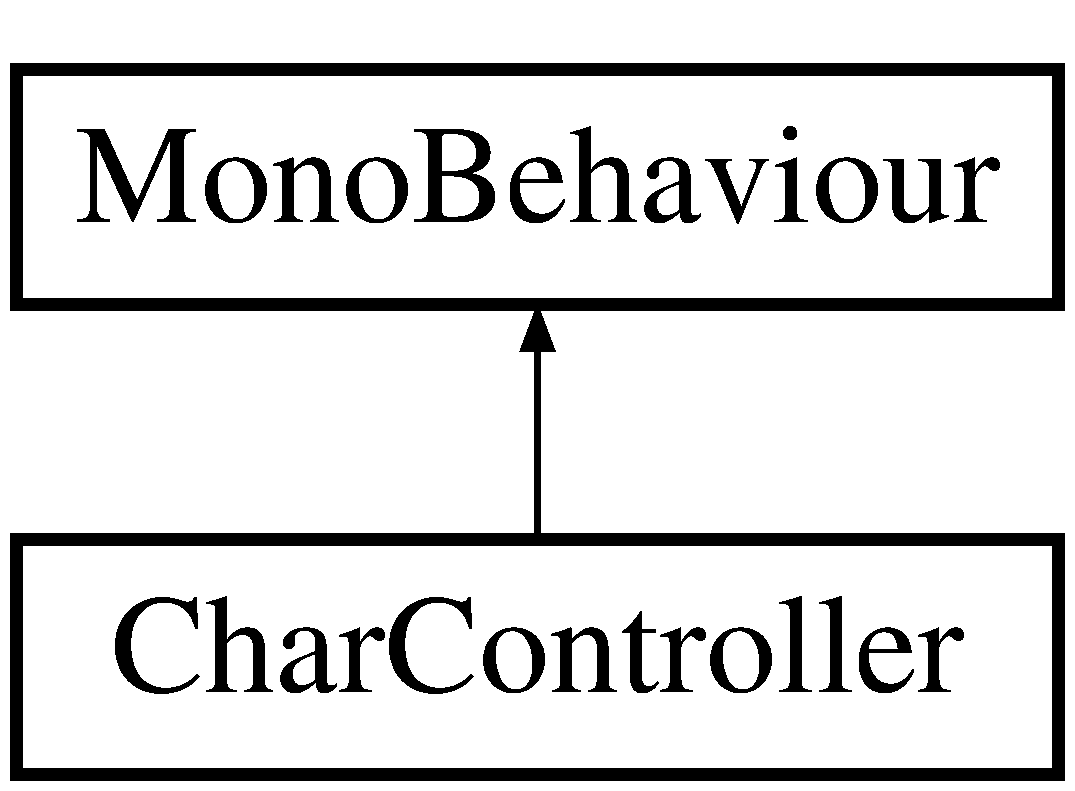
\includegraphics[height=2.000000cm]{class_char_controller}
\end{center}
\end{figure}
\subsection*{Public Attributes}
\begin{DoxyCompactItemize}
\item 
\mbox{\Hypertarget{class_char_controller_a61830f88f881dd25a5d4e399c08b3207}\label{class_char_controller_a61830f88f881dd25a5d4e399c08b3207}} 
\mbox{\hyperlink{class_joystick}{Joystick}} {\bfseries joystick}
\end{DoxyCompactItemize}


The documentation for this class was generated from the following file\+:\begin{DoxyCompactItemize}
\item 
Iso\+Chai/\+Assets/Char\+Controller.\+cs\end{DoxyCompactItemize}

\hypertarget{class_tiled2_unity_1_1_circle_object}{}\section{Tiled2\+Unity.\+Circle\+Object Class Reference}
\label{class_tiled2_unity_1_1_circle_object}\index{Tiled2\+Unity.\+Circle\+Object@{Tiled2\+Unity.\+Circle\+Object}}
Inheritance diagram for Tiled2\+Unity.\+Circle\+Object\+:\begin{figure}[H]
\begin{center}
\leavevmode
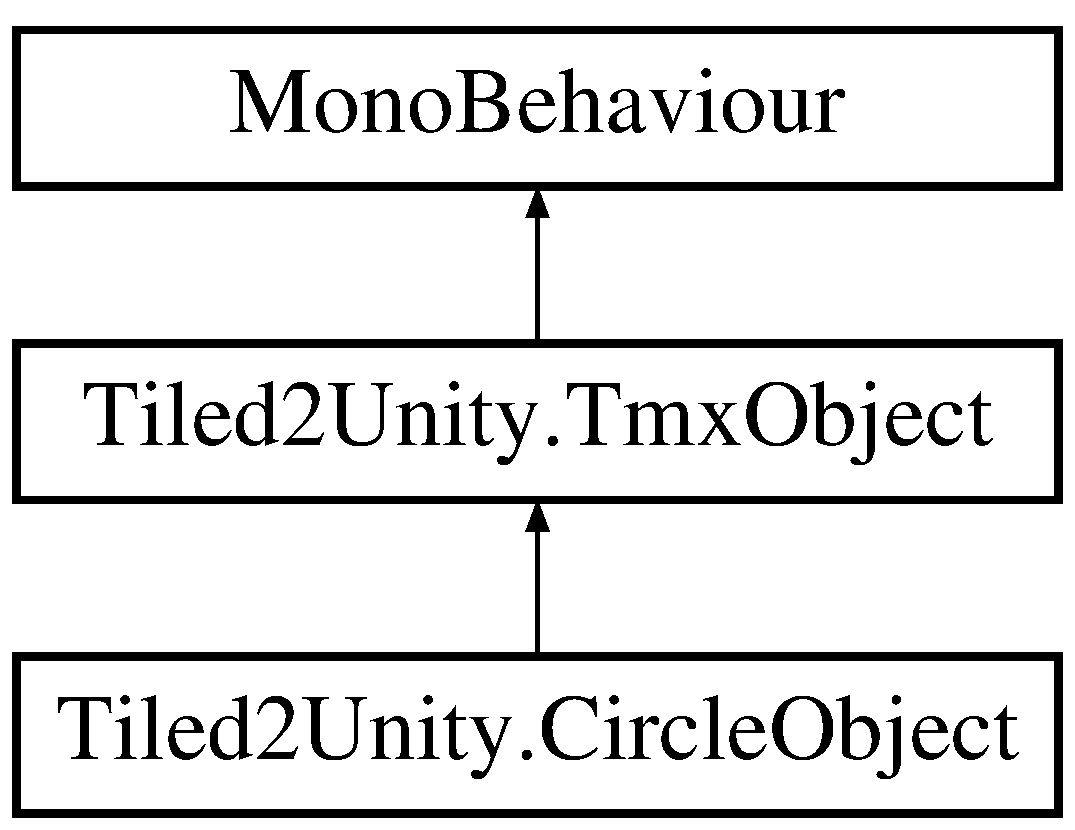
\includegraphics[height=3.000000cm]{class_tiled2_unity_1_1_circle_object}
\end{center}
\end{figure}
\subsection*{Additional Inherited Members}


The documentation for this class was generated from the following file\+:\begin{DoxyCompactItemize}
\item 
D\+:/\+Users/\+Bennett/\+Desktop/\+School/\+E\+E\+C\+S\+\_\+448/\+Catch-\/the-\/\+Bus/\+Iso\+Chai/\+Assets/\+Tiled2\+Unity/\+Scripts/\+Runtime/Circle\+Object.\+cs\end{DoxyCompactItemize}

\hypertarget{classcube}{}\section{cube Class Reference}
\label{classcube}\index{cube@{cube}}
Inheritance diagram for cube\+:\begin{figure}[H]
\begin{center}
\leavevmode
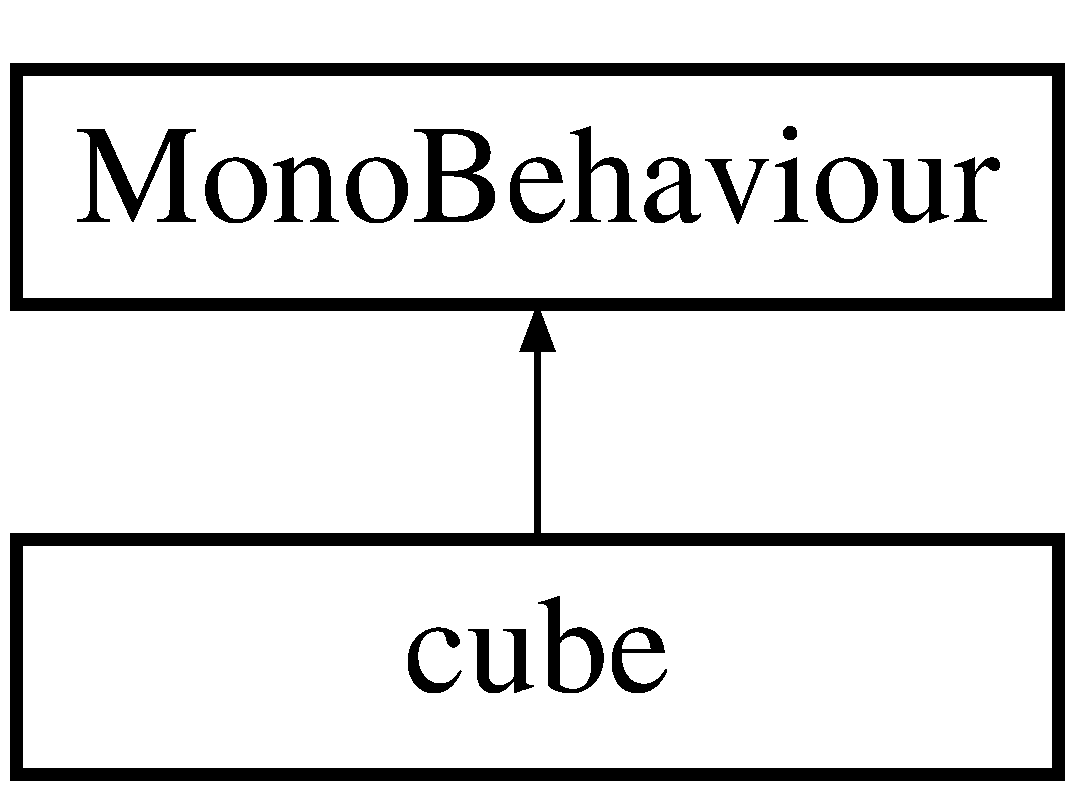
\includegraphics[height=2.000000cm]{classcube}
\end{center}
\end{figure}
\subsection*{Public Attributes}
\begin{DoxyCompactItemize}
\item 
\mbox{\Hypertarget{classcube_a07418155a0ab3c3208d92dd5d218ead4}\label{classcube_a07418155a0ab3c3208d92dd5d218ead4}} 
float {\bfseries move\+Speed}
\end{DoxyCompactItemize}


The documentation for this class was generated from the following file\+:\begin{DoxyCompactItemize}
\item 
Iso\+Chai/\+Assets/\+Tiled2\+Unity/\+Materials/cube.\+cs\end{DoxyCompactItemize}

\hypertarget{class_tiled2_unity_1_1_custom_tiled_importer_attribute}{}\section{Tiled2\+Unity.\+Custom\+Tiled\+Importer\+Attribute Class Reference}
\label{class_tiled2_unity_1_1_custom_tiled_importer_attribute}\index{Tiled2\+Unity.\+Custom\+Tiled\+Importer\+Attribute@{Tiled2\+Unity.\+Custom\+Tiled\+Importer\+Attribute}}
Inheritance diagram for Tiled2\+Unity.\+Custom\+Tiled\+Importer\+Attribute\+:\begin{figure}[H]
\begin{center}
\leavevmode
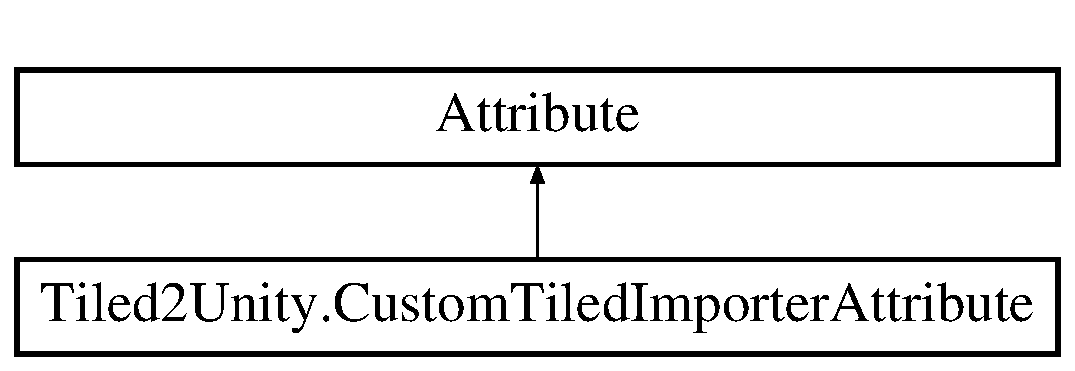
\includegraphics[height=2.000000cm]{class_tiled2_unity_1_1_custom_tiled_importer_attribute}
\end{center}
\end{figure}
\subsection*{Properties}
\begin{DoxyCompactItemize}
\item 
\mbox{\Hypertarget{class_tiled2_unity_1_1_custom_tiled_importer_attribute_ad1ed82004dd88b76c48c01094e871752}\label{class_tiled2_unity_1_1_custom_tiled_importer_attribute_ad1ed82004dd88b76c48c01094e871752}} 
int {\bfseries Order}\hspace{0.3cm}{\ttfamily  \mbox{[}get, set\mbox{]}}
\end{DoxyCompactItemize}


The documentation for this class was generated from the following file\+:\begin{DoxyCompactItemize}
\item 
Iso\+Chai/\+Assets/\+Tiled2\+Unity/\+Scripts/\+Editor/Custom\+Tiled\+Importer\+Attribute.\+cs\end{DoxyCompactItemize}

\hypertarget{class_fixed_joystick}{}\section{Fixed\+Joystick Class Reference}
\label{class_fixed_joystick}\index{Fixed\+Joystick@{Fixed\+Joystick}}
Inheritance diagram for Fixed\+Joystick\+:\begin{figure}[H]
\begin{center}
\leavevmode
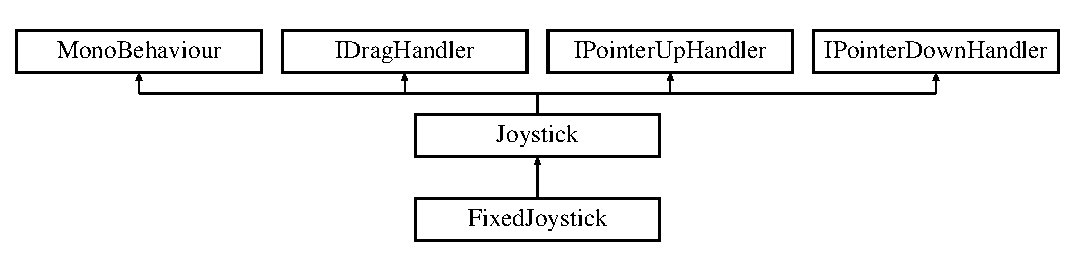
\includegraphics[height=3.000000cm]{class_fixed_joystick}
\end{center}
\end{figure}
\subsection*{Public Member Functions}
\begin{DoxyCompactItemize}
\item 
\mbox{\Hypertarget{class_fixed_joystick_a3608a6ae388b2718af9b91155d86eea5}\label{class_fixed_joystick_a3608a6ae388b2718af9b91155d86eea5}} 
override void {\bfseries On\+Drag} (Pointer\+Event\+Data event\+Data)
\item 
\mbox{\Hypertarget{class_fixed_joystick_a2e6be1323f094b36b40f820cc326c06f}\label{class_fixed_joystick_a2e6be1323f094b36b40f820cc326c06f}} 
override void {\bfseries On\+Pointer\+Down} (Pointer\+Event\+Data event\+Data)
\item 
\mbox{\Hypertarget{class_fixed_joystick_acebb0623f5935bf101b718aacb5b5ac3}\label{class_fixed_joystick_acebb0623f5935bf101b718aacb5b5ac3}} 
override void {\bfseries On\+Pointer\+Up} (Pointer\+Event\+Data event\+Data)
\end{DoxyCompactItemize}
\subsection*{Additional Inherited Members}


The documentation for this class was generated from the following file\+:\begin{DoxyCompactItemize}
\item 
D\+:/\+Users/\+Bennett/\+Desktop/\+School/\+E\+E\+C\+S\+\_\+448/\+Catch-\/the-\/\+Bus/\+Iso\+Chai/\+Assets/\+Virtual Joystick Pack/\+Scripts/\+Joysticks/Fixed\+Joystick.\+cs\end{DoxyCompactItemize}

\hypertarget{class_floating_joystick}{}\section{Floating\+Joystick Class Reference}
\label{class_floating_joystick}\index{Floating\+Joystick@{Floating\+Joystick}}
Inheritance diagram for Floating\+Joystick\+:\begin{figure}[H]
\begin{center}
\leavevmode
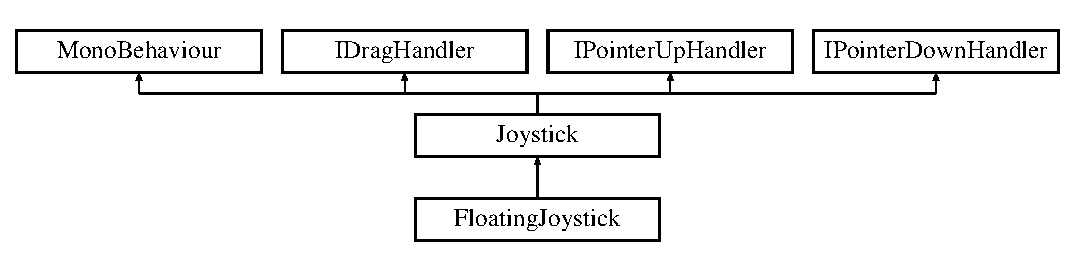
\includegraphics[height=3.000000cm]{class_floating_joystick}
\end{center}
\end{figure}
\subsection*{Public Member Functions}
\begin{DoxyCompactItemize}
\item 
\mbox{\Hypertarget{class_floating_joystick_a522d320721f122a99ba50701447eaf1f}\label{class_floating_joystick_a522d320721f122a99ba50701447eaf1f}} 
override void {\bfseries On\+Drag} (Pointer\+Event\+Data event\+Data)
\item 
\mbox{\Hypertarget{class_floating_joystick_ae6793e17984d80f589de93afbd697bb9}\label{class_floating_joystick_ae6793e17984d80f589de93afbd697bb9}} 
override void {\bfseries On\+Pointer\+Down} (Pointer\+Event\+Data event\+Data)
\item 
\mbox{\Hypertarget{class_floating_joystick_af651ab0edbcbd7f644b81035c3e66d12}\label{class_floating_joystick_af651ab0edbcbd7f644b81035c3e66d12}} 
override void {\bfseries On\+Pointer\+Up} (Pointer\+Event\+Data event\+Data)
\end{DoxyCompactItemize}
\subsection*{Additional Inherited Members}


The documentation for this class was generated from the following file\+:\begin{DoxyCompactItemize}
\item 
Iso\+Chai/\+Assets/\+Virtual Joystick Pack/\+Scripts/\+Joysticks/Floating\+Joystick.\+cs\end{DoxyCompactItemize}

\hypertarget{class_tiled2_unity_1_1_g_p_u_instancing}{}\section{Tiled2\+Unity.\+G\+P\+U\+Instancing Class Reference}
\label{class_tiled2_unity_1_1_g_p_u_instancing}\index{Tiled2\+Unity.\+G\+P\+U\+Instancing@{Tiled2\+Unity.\+G\+P\+U\+Instancing}}
Inheritance diagram for Tiled2\+Unity.\+G\+P\+U\+Instancing\+:\begin{figure}[H]
\begin{center}
\leavevmode
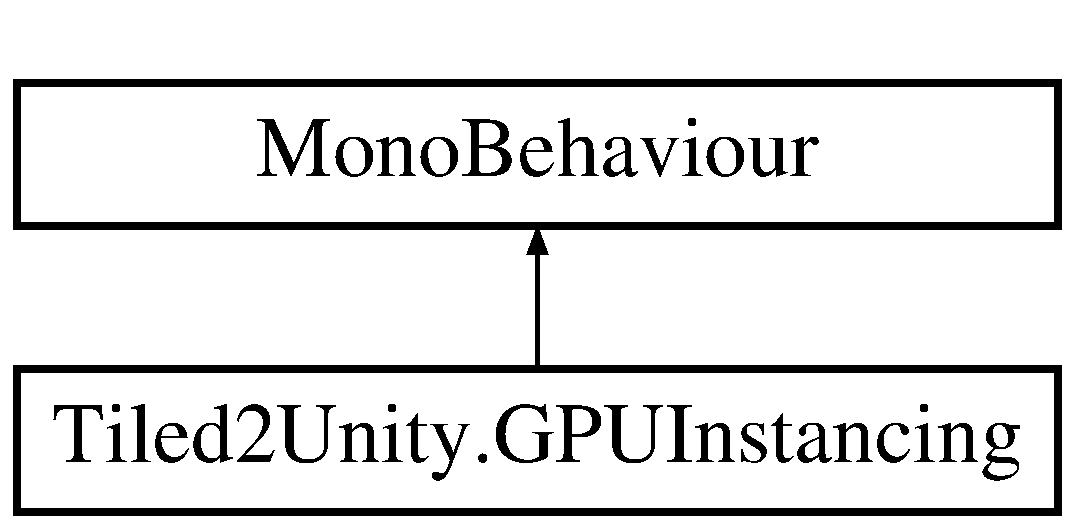
\includegraphics[height=2.000000cm]{class_tiled2_unity_1_1_g_p_u_instancing}
\end{center}
\end{figure}
\subsection*{Public Attributes}
\begin{DoxyCompactItemize}
\item 
\mbox{\Hypertarget{class_tiled2_unity_1_1_g_p_u_instancing_a3d9886fd691a897ed1ed57bd247e6e18}\label{class_tiled2_unity_1_1_g_p_u_instancing_a3d9886fd691a897ed1ed57bd247e6e18}} 
float {\bfseries Opacity} = 1.\+0f
\end{DoxyCompactItemize}


The documentation for this class was generated from the following file\+:\begin{DoxyCompactItemize}
\item 
D\+:/\+Users/\+Bennett/\+Desktop/\+School/\+E\+E\+C\+S\+\_\+448/\+Catch-\/the-\/\+Bus/\+Iso\+Chai/\+Assets/\+Tiled2\+Unity/\+Scripts/\+Runtime/G\+P\+U\+Instancing.\+cs\end{DoxyCompactItemize}

\hypertarget{class_tiled2_unity_1_1_group_layer}{}\section{Tiled2\+Unity.\+Group\+Layer Class Reference}
\label{class_tiled2_unity_1_1_group_layer}\index{Tiled2\+Unity.\+Group\+Layer@{Tiled2\+Unity.\+Group\+Layer}}
Inheritance diagram for Tiled2\+Unity.\+Group\+Layer\+:\begin{figure}[H]
\begin{center}
\leavevmode
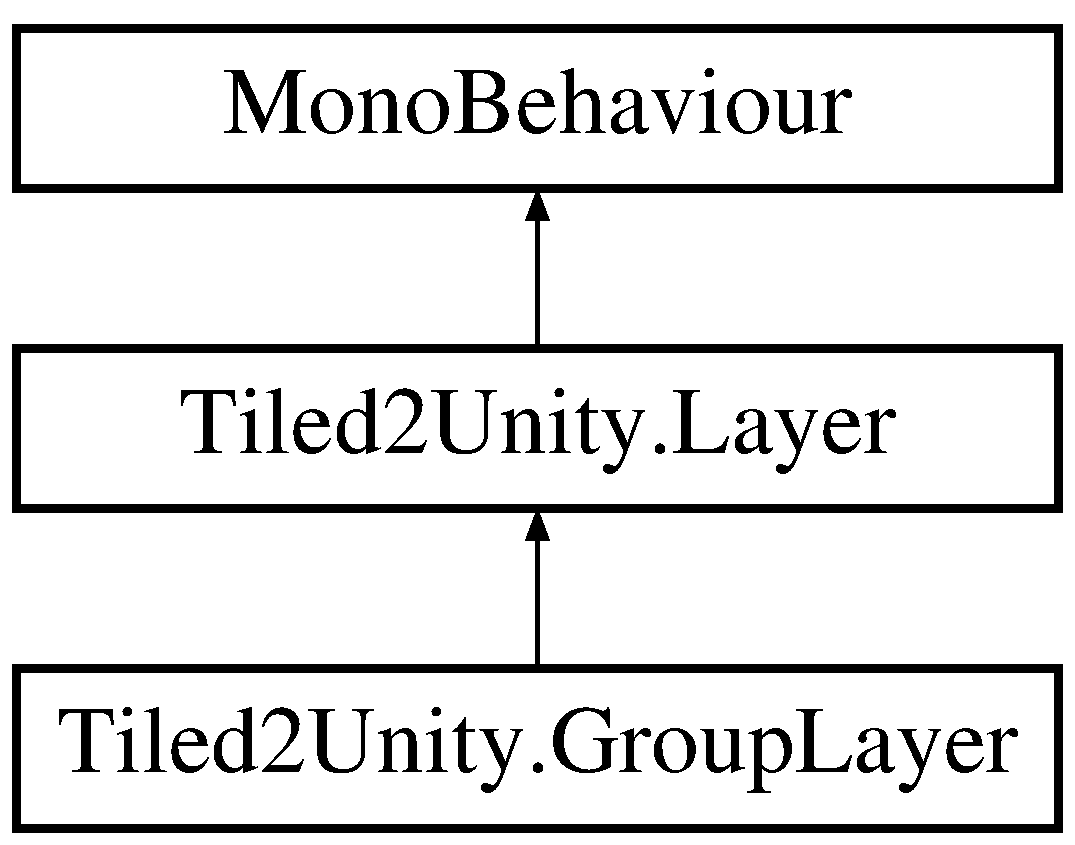
\includegraphics[height=3.000000cm]{class_tiled2_unity_1_1_group_layer}
\end{center}
\end{figure}
\subsection*{Additional Inherited Members}


The documentation for this class was generated from the following file\+:\begin{DoxyCompactItemize}
\item 
Iso\+Chai/\+Assets/\+Tiled2\+Unity/\+Scripts/\+Runtime/Group\+Layer.\+cs\end{DoxyCompactItemize}

\hypertarget{interface_tiled2_unity_1_1_i_custom_tiled_importer}{}\section{Tiled2\+Unity.\+I\+Custom\+Tiled\+Importer Interface Reference}
\label{interface_tiled2_unity_1_1_i_custom_tiled_importer}\index{Tiled2\+Unity.\+I\+Custom\+Tiled\+Importer@{Tiled2\+Unity.\+I\+Custom\+Tiled\+Importer}}
\subsection*{Public Member Functions}
\begin{DoxyCompactItemize}
\item 
\mbox{\Hypertarget{interface_tiled2_unity_1_1_i_custom_tiled_importer_af4c9e46be5df1af5cbd4ac2114c8fcd8}\label{interface_tiled2_unity_1_1_i_custom_tiled_importer_af4c9e46be5df1af5cbd4ac2114c8fcd8}} 
void {\bfseries Handle\+Custom\+Properties} (Game\+Object game\+Object, I\+Dictionary$<$ string, string $>$ custom\+Properties)
\item 
\mbox{\Hypertarget{interface_tiled2_unity_1_1_i_custom_tiled_importer_af2334f3b1851b0f84ba8b1035333cffd}\label{interface_tiled2_unity_1_1_i_custom_tiled_importer_af2334f3b1851b0f84ba8b1035333cffd}} 
void {\bfseries Customize\+Prefab} (Game\+Object prefab)
\end{DoxyCompactItemize}


The documentation for this interface was generated from the following file\+:\begin{DoxyCompactItemize}
\item 
D\+:/\+Users/\+Bennett/\+Desktop/\+School/\+E\+E\+C\+S\+\_\+448/\+Catch-\/the-\/\+Bus/\+Iso\+Chai/\+Assets/\+Tiled2\+Unity/\+Scripts/\+Editor/I\+Custom\+Tiled\+Importer.\+cs\end{DoxyCompactItemize}

\hypertarget{class_tiled2_unity_1_1_import_behaviour}{}\section{Tiled2\+Unity.\+Import\+Behaviour Class Reference}
\label{class_tiled2_unity_1_1_import_behaviour}\index{Tiled2\+Unity.\+Import\+Behaviour@{Tiled2\+Unity.\+Import\+Behaviour}}
Inheritance diagram for Tiled2\+Unity.\+Import\+Behaviour\+:\begin{figure}[H]
\begin{center}
\leavevmode
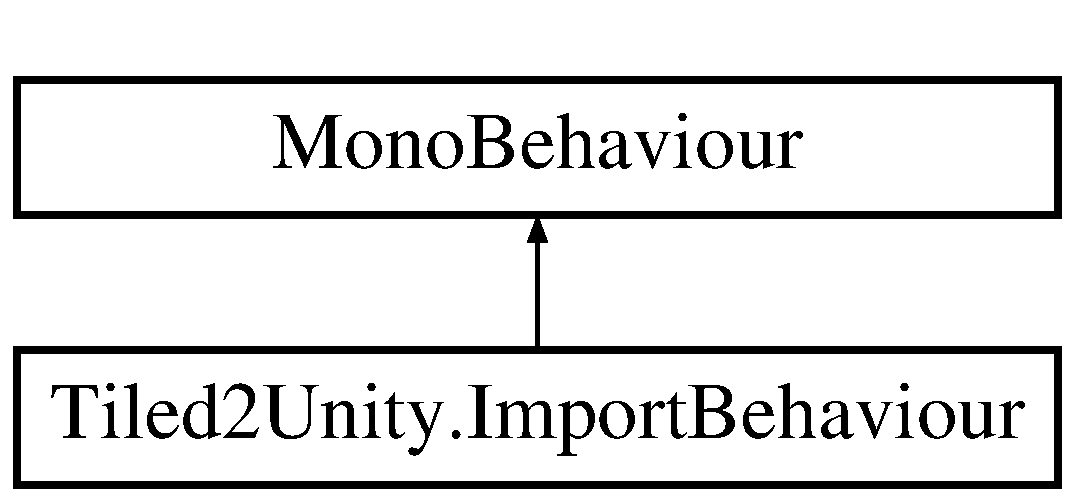
\includegraphics[height=2.000000cm]{class_tiled2_unity_1_1_import_behaviour}
\end{center}
\end{figure}
\subsection*{Public Attributes}
\begin{DoxyCompactItemize}
\item 
\mbox{\Hypertarget{class_tiled2_unity_1_1_import_behaviour_a8562ebe80cd0f8e44403ec3eb604ddfd}\label{class_tiled2_unity_1_1_import_behaviour_a8562ebe80cd0f8e44403ec3eb604ddfd}} 
string {\bfseries Tiled2\+Unity\+Xml\+Path} = \char`\"{}\char`\"{}
\item 
\mbox{\Hypertarget{class_tiled2_unity_1_1_import_behaviour_ad8c0fb24237c9f5fa29ebb4946420805}\label{class_tiled2_unity_1_1_import_behaviour_ad8c0fb24237c9f5fa29ebb4946420805}} 
string {\bfseries Exporter\+Tiled2\+Unity\+Version} = \char`\"{}tiled2unity.\+version.\+not.\+set\char`\"{}
\end{DoxyCompactItemize}


The documentation for this class was generated from the following file\+:\begin{DoxyCompactItemize}
\item 
Iso\+Chai/\+Assets/\+Tiled2\+Unity/\+Scripts/\+Runtime/Import\+Behaviour.\+cs\end{DoxyCompactItemize}

\hypertarget{class_tiled2_unity_1_1_import_tiled2_unity}{}\section{Tiled2\+Unity.\+Import\+Tiled2\+Unity Class Reference}
\label{class_tiled2_unity_1_1_import_tiled2_unity}\index{Tiled2\+Unity.\+Import\+Tiled2\+Unity@{Tiled2\+Unity.\+Import\+Tiled2\+Unity}}
Inheritance diagram for Tiled2\+Unity.\+Import\+Tiled2\+Unity\+:\begin{figure}[H]
\begin{center}
\leavevmode
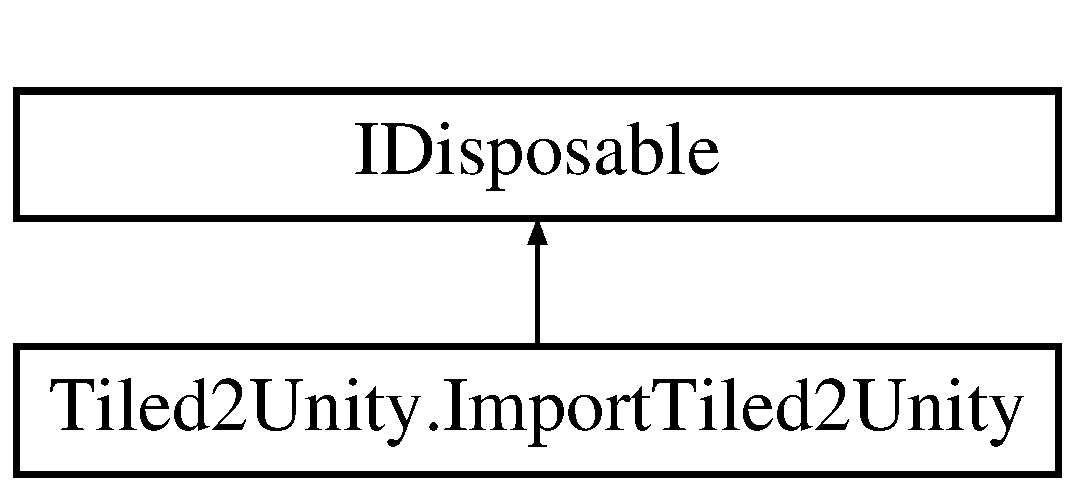
\includegraphics[height=2.000000cm]{class_tiled2_unity_1_1_import_tiled2_unity}
\end{center}
\end{figure}
\subsection*{Public Member Functions}
\begin{DoxyCompactItemize}
\item 
\mbox{\Hypertarget{class_tiled2_unity_1_1_import_tiled2_unity_aa32997e829fe81a1a7b8b5ede4a12133}\label{class_tiled2_unity_1_1_import_tiled2_unity_aa32997e829fe81a1a7b8b5ede4a12133}} 
{\bfseries Import\+Tiled2\+Unity} (string file)
\item 
\mbox{\Hypertarget{class_tiled2_unity_1_1_import_tiled2_unity_ad87a2791643d8271785ca5088f51ff11}\label{class_tiled2_unity_1_1_import_tiled2_unity_ad87a2791643d8271785ca5088f51ff11}} 
bool {\bfseries Is\+Tiled2\+Unity\+File} ()
\item 
\mbox{\Hypertarget{class_tiled2_unity_1_1_import_tiled2_unity_a00ff3f8735692125bfb3e2aa20c5a2b0}\label{class_tiled2_unity_1_1_import_tiled2_unity_a00ff3f8735692125bfb3e2aa20c5a2b0}} 
bool {\bfseries Is\+Tiled2\+Unity\+Texture} ()
\item 
\mbox{\Hypertarget{class_tiled2_unity_1_1_import_tiled2_unity_aeaaf1f5bf827d2368f7307f9a1ecd233}\label{class_tiled2_unity_1_1_import_tiled2_unity_aeaaf1f5bf827d2368f7307f9a1ecd233}} 
bool {\bfseries Is\+Tiled2\+Unity\+Material} ()
\item 
\mbox{\Hypertarget{class_tiled2_unity_1_1_import_tiled2_unity_a9a7be37df827bb2135724cdb781282c0}\label{class_tiled2_unity_1_1_import_tiled2_unity_a9a7be37df827bb2135724cdb781282c0}} 
bool {\bfseries Is\+Tiled2\+Unity\+Wavefront\+Obj} ()
\item 
\mbox{\Hypertarget{class_tiled2_unity_1_1_import_tiled2_unity_acb38dc0527118d7b589d7e193feafe61}\label{class_tiled2_unity_1_1_import_tiled2_unity_acb38dc0527118d7b589d7e193feafe61}} 
bool {\bfseries Is\+Tiled2\+Unity\+Prefab} ()
\item 
\mbox{\Hypertarget{class_tiled2_unity_1_1_import_tiled2_unity_a66db37d79d3768748059338f5281a4fa}\label{class_tiled2_unity_1_1_import_tiled2_unity_a66db37d79d3768748059338f5281a4fa}} 
string {\bfseries Get\+Mesh\+Asset\+Path} (string map\+Name, string mesh\+Name)
\item 
\mbox{\Hypertarget{class_tiled2_unity_1_1_import_tiled2_unity_a8eccce3bc913c345c5bec35c38daa2c1}\label{class_tiled2_unity_1_1_import_tiled2_unity_a8eccce3bc913c345c5bec35c38daa2c1}} 
string {\bfseries Make\+Material\+Asset\+Path} (string file, bool is\+Resource)
\item 
\mbox{\Hypertarget{class_tiled2_unity_1_1_import_tiled2_unity_a36d076495b6d091959683c301a04b4b2}\label{class_tiled2_unity_1_1_import_tiled2_unity_a36d076495b6d091959683c301a04b4b2}} 
string {\bfseries Get\+Existing\+Material\+Asset\+Path} (string file)
\item 
\mbox{\Hypertarget{class_tiled2_unity_1_1_import_tiled2_unity_ab518dfb851c9b8ae02c942d568e12326}\label{class_tiled2_unity_1_1_import_tiled2_unity_ab518dfb851c9b8ae02c942d568e12326}} 
Text\+Asset {\bfseries Get\+Tiled2\+Unity\+Text\+Asset} ()
\item 
\mbox{\Hypertarget{class_tiled2_unity_1_1_import_tiled2_unity_af199d19db0fbbe7f5836633e6fa8f798}\label{class_tiled2_unity_1_1_import_tiled2_unity_af199d19db0fbbe7f5836633e6fa8f798}} 
string {\bfseries Get\+Texture\+Asset\+Path} (string filename)
\item 
\mbox{\Hypertarget{class_tiled2_unity_1_1_import_tiled2_unity_ac1f0dc4fd45b213327c3085bc0c38038}\label{class_tiled2_unity_1_1_import_tiled2_unity_ac1f0dc4fd45b213327c3085bc0c38038}} 
string {\bfseries Get\+Prefab\+Asset\+Path} (string name, bool is\+Resource, string extra\+Path)
\item 
\mbox{\Hypertarget{class_tiled2_unity_1_1_import_tiled2_unity_aa2193f54b0c54f4be6f7077668061fce}\label{class_tiled2_unity_1_1_import_tiled2_unity_aa2193f54b0c54f4be6f7077668061fce}} 
void {\bfseries Dispose} ()
\item 
\mbox{\Hypertarget{class_tiled2_unity_1_1_import_tiled2_unity_abe871380459e1120c54c920b63725a5a}\label{class_tiled2_unity_1_1_import_tiled2_unity_abe871380459e1120c54c920b63725a5a}} 
void {\bfseries Material\+Imported} (string material\+Path)
\item 
\mbox{\Hypertarget{class_tiled2_unity_1_1_import_tiled2_unity_a40bfd0211731100d0d36d8ad94f2974e}\label{class_tiled2_unity_1_1_import_tiled2_unity_a40bfd0211731100d0d36d8ad94f2974e}} 
Unity\+Engine.\+Material {\bfseries Fix\+Material\+For\+Mesh\+Renderer} (string obj\+Name, Renderer renderer)
\item 
\mbox{\Hypertarget{class_tiled2_unity_1_1_import_tiled2_unity_a58536db75e369597819f10abd676f74c}\label{class_tiled2_unity_1_1_import_tiled2_unity_a58536db75e369597819f10abd676f74c}} 
void {\bfseries Mesh\+Imported} (string obj\+Path)
\item 
\mbox{\Hypertarget{class_tiled2_unity_1_1_import_tiled2_unity_a76f2e7873d1ca6242e309de2ee8c6955}\label{class_tiled2_unity_1_1_import_tiled2_unity_a76f2e7873d1ca6242e309de2ee8c6955}} 
void {\bfseries Prefab\+Imported} (string prefab\+Path)
\item 
\mbox{\Hypertarget{class_tiled2_unity_1_1_import_tiled2_unity_ad4f3e0e6fa83359316fa547ceae92b8c}\label{class_tiled2_unity_1_1_import_tiled2_unity_ad4f3e0e6fa83359316fa547ceae92b8c}} 
void {\bfseries Texture\+Imported} (string texture\+Path)
\item 
\mbox{\Hypertarget{class_tiled2_unity_1_1_import_tiled2_unity_ab59e3ca83b03c07989eec10f347e96bf}\label{class_tiled2_unity_1_1_import_tiled2_unity_ab59e3ca83b03c07989eec10f347e96bf}} 
void {\bfseries Import\+Begin} (string xml\+Path, \mbox{\hyperlink{class_tiled2_unity_1_1_import_tiled2_unity}{Tiled2\+Unity.\+Import\+Tiled2\+Unity}} import\+Tiled2\+Unity)
\end{DoxyCompactItemize}


The documentation for this class was generated from the following files\+:\begin{DoxyCompactItemize}
\item 
D\+:/\+Users/\+Bennett/\+Desktop/\+School/\+E\+E\+C\+S\+\_\+448/\+Catch-\/the-\/\+Bus/\+Iso\+Chai/\+Assets/\+Tiled2\+Unity/\+Scripts/\+Editor/Import\+Tiled2\+Unity.\+cs\item 
D\+:/\+Users/\+Bennett/\+Desktop/\+School/\+E\+E\+C\+S\+\_\+448/\+Catch-\/the-\/\+Bus/\+Iso\+Chai/\+Assets/\+Tiled2\+Unity/\+Scripts/\+Editor/Import\+Tiled2\+Unity.\+Material.\+cs\item 
D\+:/\+Users/\+Bennett/\+Desktop/\+School/\+E\+E\+C\+S\+\_\+448/\+Catch-\/the-\/\+Bus/\+Iso\+Chai/\+Assets/\+Tiled2\+Unity/\+Scripts/\+Editor/Import\+Tiled2\+Unity.\+Mesh.\+cs\item 
D\+:/\+Users/\+Bennett/\+Desktop/\+School/\+E\+E\+C\+S\+\_\+448/\+Catch-\/the-\/\+Bus/\+Iso\+Chai/\+Assets/\+Tiled2\+Unity/\+Scripts/\+Editor/Import\+Tiled2\+Unity.\+Prefab.\+cs\item 
D\+:/\+Users/\+Bennett/\+Desktop/\+School/\+E\+E\+C\+S\+\_\+448/\+Catch-\/the-\/\+Bus/\+Iso\+Chai/\+Assets/\+Tiled2\+Unity/\+Scripts/\+Editor/Import\+Tiled2\+Unity.\+Texture.\+cs\item 
D\+:/\+Users/\+Bennett/\+Desktop/\+School/\+E\+E\+C\+S\+\_\+448/\+Catch-\/the-\/\+Bus/\+Iso\+Chai/\+Assets/\+Tiled2\+Unity/\+Scripts/\+Editor/Import\+Tiled2\+Unity.\+Xml.\+cs\end{DoxyCompactItemize}

\hypertarget{class_tiled2_unity_1_1_import_utils}{}\section{Tiled2\+Unity.\+Import\+Utils Class Reference}
\label{class_tiled2_unity_1_1_import_utils}\index{Tiled2\+Unity.\+Import\+Utils@{Tiled2\+Unity.\+Import\+Utils}}
\subsection*{Static Public Member Functions}
\begin{DoxyCompactItemize}
\item 
\mbox{\Hypertarget{class_tiled2_unity_1_1_import_utils_a6b9c8d7811ab60c57a1f706dfc4909c3}\label{class_tiled2_unity_1_1_import_utils_a6b9c8d7811ab60c57a1f706dfc4909c3}} 
static string {\bfseries Get\+Attribute\+As\+String} (X\+Element elem, string attr\+Name)
\item 
\mbox{\Hypertarget{class_tiled2_unity_1_1_import_utils_a963cc485c7518ba85e384b744e1ed552}\label{class_tiled2_unity_1_1_import_utils_a963cc485c7518ba85e384b744e1ed552}} 
static string {\bfseries Get\+Attribute\+As\+String} (X\+Element elem, string attr\+Name, string default\+Value)
\item 
\mbox{\Hypertarget{class_tiled2_unity_1_1_import_utils_a91b971fb856c5458a556dead9022b5b3}\label{class_tiled2_unity_1_1_import_utils_a91b971fb856c5458a556dead9022b5b3}} 
static int {\bfseries Get\+Attribute\+As\+Int} (X\+Element elem, string attr\+Name)
\item 
\mbox{\Hypertarget{class_tiled2_unity_1_1_import_utils_aeef489bd7347636aebc95e1efa4520c4}\label{class_tiled2_unity_1_1_import_utils_aeef489bd7347636aebc95e1efa4520c4}} 
static int {\bfseries Get\+Attribute\+As\+Int} (X\+Element elem, string attr\+Name, int default\+Value)
\item 
\mbox{\Hypertarget{class_tiled2_unity_1_1_import_utils_a381761e5855cd4dc534522c0a39158a5}\label{class_tiled2_unity_1_1_import_utils_a381761e5855cd4dc534522c0a39158a5}} 
static float {\bfseries Get\+Attribute\+As\+Float} (X\+Element elem, string attr\+Name)
\item 
\mbox{\Hypertarget{class_tiled2_unity_1_1_import_utils_ac8038d177230fe92c297c4212479f11b}\label{class_tiled2_unity_1_1_import_utils_ac8038d177230fe92c297c4212479f11b}} 
static float {\bfseries Get\+Attribute\+As\+Float} (X\+Element elem, string attr\+Name, float default\+Value)
\item 
\mbox{\Hypertarget{class_tiled2_unity_1_1_import_utils_ad07d814f168a62de77c6feb055b28fc6}\label{class_tiled2_unity_1_1_import_utils_ad07d814f168a62de77c6feb055b28fc6}} 
static bool {\bfseries Get\+Attribute\+As\+Boolean} (X\+Element elem, string attr\+Name)
\item 
\mbox{\Hypertarget{class_tiled2_unity_1_1_import_utils_a03cc67fb90080b345bcae6a3f4af6112}\label{class_tiled2_unity_1_1_import_utils_a03cc67fb90080b345bcae6a3f4af6112}} 
static bool {\bfseries Get\+Attribute\+As\+Boolean} (X\+Element elem, string attr\+Name, bool default\+Value)
\item 
\mbox{\Hypertarget{class_tiled2_unity_1_1_import_utils_a1bb629963e5bcce5b484d01463d79c47}\label{class_tiled2_unity_1_1_import_utils_a1bb629963e5bcce5b484d01463d79c47}} 
static T {\bfseries Get\+String\+As\+Enum$<$ T $>$} (string enum\+String)
\item 
\mbox{\Hypertarget{class_tiled2_unity_1_1_import_utils_a13f4f397b11315cd4f235195985b694c}\label{class_tiled2_unity_1_1_import_utils_a13f4f397b11315cd4f235195985b694c}} 
static T {\bfseries Get\+Attribute\+As\+Enum$<$ T $>$} (X\+Element elem, string attr\+Name)
\item 
\mbox{\Hypertarget{class_tiled2_unity_1_1_import_utils_aa49f3ec90727df791a864e99ac32ef60}\label{class_tiled2_unity_1_1_import_utils_aa49f3ec90727df791a864e99ac32ef60}} 
static string {\bfseries Get\+Attribute\+As\+Full\+Path} (X\+Element elem, string attr\+Name)
\item 
\mbox{\Hypertarget{class_tiled2_unity_1_1_import_utils_a117905bc790ba993fb51f84ebf20d26a}\label{class_tiled2_unity_1_1_import_utils_a117905bc790ba993fb51f84ebf20d26a}} 
static Color {\bfseries Get\+Attribute\+As\+Color} (X\+Element elem, string attr\+Name)
\item 
\mbox{\Hypertarget{class_tiled2_unity_1_1_import_utils_ae637054202cc20c1908d98d2b62e1927}\label{class_tiled2_unity_1_1_import_utils_ae637054202cc20c1908d98d2b62e1927}} 
static Color {\bfseries Get\+Attribute\+As\+Color} (X\+Element elem, string attr\+Name, Color default\+Value)
\item 
\mbox{\Hypertarget{class_tiled2_unity_1_1_import_utils_a11cec173605584ea154aaa5419a89234}\label{class_tiled2_unity_1_1_import_utils_a11cec173605584ea154aaa5419a89234}} 
static void {\bfseries Ready\+To\+Write} (string path)
\item 
\mbox{\Hypertarget{class_tiled2_unity_1_1_import_utils_a5e2d417ee1fb13a9e089c913752939ee}\label{class_tiled2_unity_1_1_import_utils_a5e2d417ee1fb13a9e089c913752939ee}} 
static T {\bfseries Create\+Or\+Replace\+Asset$<$ T $>$} (T asset, string path)
\item 
\mbox{\Hypertarget{class_tiled2_unity_1_1_import_utils_a1cc61166584f7ae7e358caf652cd4db7}\label{class_tiled2_unity_1_1_import_utils_a1cc61166584f7ae7e358caf652cd4db7}} 
static byte \mbox{[}$\,$\mbox{]} {\bfseries Base64\+To\+Bytes} (string base64)
\item 
\mbox{\Hypertarget{class_tiled2_unity_1_1_import_utils_a17abc9fcab7f46129163791fa9156b92}\label{class_tiled2_unity_1_1_import_utils_a17abc9fcab7f46129163791fa9156b92}} 
static string {\bfseries Base64\+To\+String} (string base64)
\end{DoxyCompactItemize}


The documentation for this class was generated from the following file\+:\begin{DoxyCompactItemize}
\item 
D\+:/\+Users/\+Bennett/\+Desktop/\+School/\+E\+E\+C\+S\+\_\+448/\+Catch-\/the-\/\+Bus/\+Iso\+Chai/\+Assets/\+Tiled2\+Unity/\+Scripts/\+Editor/Import\+Utils.\+cs\end{DoxyCompactItemize}

\hypertarget{class_joystick}{}\section{Joystick Class Reference}
\label{class_joystick}\index{Joystick@{Joystick}}
Inheritance diagram for Joystick\+:\begin{figure}[H]
\begin{center}
\leavevmode
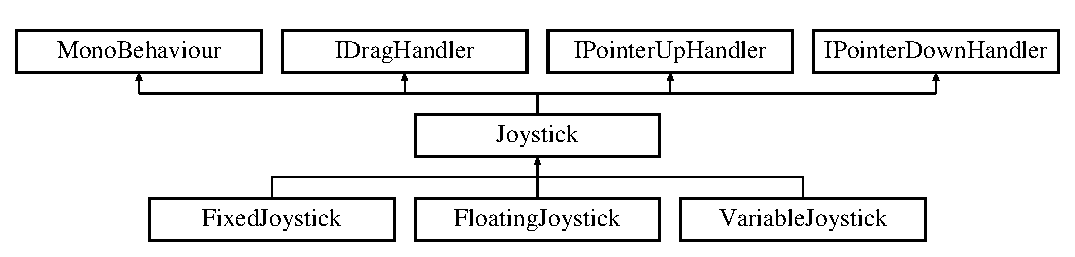
\includegraphics[height=3.000000cm]{class_joystick}
\end{center}
\end{figure}
\subsection*{Public Member Functions}
\begin{DoxyCompactItemize}
\item 
\mbox{\Hypertarget{class_joystick_a8effe0188579d5881908bd95d51b5859}\label{class_joystick_a8effe0188579d5881908bd95d51b5859}} 
virtual void {\bfseries On\+Drag} (Pointer\+Event\+Data event\+Data)
\item 
\mbox{\Hypertarget{class_joystick_a5e7b57028c248da4e06528c90cf37721}\label{class_joystick_a5e7b57028c248da4e06528c90cf37721}} 
virtual void {\bfseries On\+Pointer\+Down} (Pointer\+Event\+Data event\+Data)
\item 
\mbox{\Hypertarget{class_joystick_ad56badf3ee242443cb4f5940d6b00701}\label{class_joystick_ad56badf3ee242443cb4f5940d6b00701}} 
virtual void {\bfseries On\+Pointer\+Up} (Pointer\+Event\+Data event\+Data)
\end{DoxyCompactItemize}
\subsection*{Public Attributes}
\begin{DoxyCompactItemize}
\item 
\mbox{\Hypertarget{class_joystick_aae5668c7a6a91fb382537b388da5ec40}\label{class_joystick_aae5668c7a6a91fb382537b388da5ec40}} 
float {\bfseries handle\+Limit} = 1f
\item 
\mbox{\Hypertarget{class_joystick_ada95319ba9975f743d6f074cbd0d7b83}\label{class_joystick_ada95319ba9975f743d6f074cbd0d7b83}} 
Joystick\+Mode {\bfseries joystick\+Mode} = Joystick\+Mode.\+All\+Axis
\item 
\mbox{\Hypertarget{class_joystick_a893fe373ca256b507d68dee82d51b389}\label{class_joystick_a893fe373ca256b507d68dee82d51b389}} 
Rect\+Transform {\bfseries background}
\item 
\mbox{\Hypertarget{class_joystick_aca64551fcfa66b5a9558d80a64b426c8}\label{class_joystick_aca64551fcfa66b5a9558d80a64b426c8}} 
Rect\+Transform {\bfseries handle}
\end{DoxyCompactItemize}
\subsection*{Protected Member Functions}
\begin{DoxyCompactItemize}
\item 
\mbox{\Hypertarget{class_joystick_a1a25fbacf5d6c6275abda7f8c29d0e0c}\label{class_joystick_a1a25fbacf5d6c6275abda7f8c29d0e0c}} 
void {\bfseries Clamp\+Joystick} ()
\end{DoxyCompactItemize}
\subsection*{Protected Attributes}
\begin{DoxyCompactItemize}
\item 
\mbox{\Hypertarget{class_joystick_a8b1dd8b1874e78a0a2781a847c2cd768}\label{class_joystick_a8b1dd8b1874e78a0a2781a847c2cd768}} 
Vector2 {\bfseries input\+Vector} = Vector2.\+zero
\end{DoxyCompactItemize}
\subsection*{Properties}
\begin{DoxyCompactItemize}
\item 
\mbox{\Hypertarget{class_joystick_aa96a7d4d3f9c4b3d79747b0fb4a0d4f7}\label{class_joystick_aa96a7d4d3f9c4b3d79747b0fb4a0d4f7}} 
float {\bfseries Horizontal}\hspace{0.3cm}{\ttfamily  \mbox{[}get\mbox{]}}
\item 
\mbox{\Hypertarget{class_joystick_aaa4ab10e8e5f17095b192a64eb3f65c9}\label{class_joystick_aaa4ab10e8e5f17095b192a64eb3f65c9}} 
float {\bfseries Vertical}\hspace{0.3cm}{\ttfamily  \mbox{[}get\mbox{]}}
\item 
\mbox{\Hypertarget{class_joystick_a7c7c6bc3ace9d2014e2b7f8234e979ea}\label{class_joystick_a7c7c6bc3ace9d2014e2b7f8234e979ea}} 
Vector2 {\bfseries Direction}\hspace{0.3cm}{\ttfamily  \mbox{[}get\mbox{]}}
\end{DoxyCompactItemize}


The documentation for this class was generated from the following file\+:\begin{DoxyCompactItemize}
\item 
D\+:/\+Users/\+Bennett/\+Desktop/\+School/\+E\+E\+C\+S\+\_\+448/\+Catch-\/the-\/\+Bus/\+Iso\+Chai/\+Assets/\+Virtual Joystick Pack/\+Scripts/\+Base/Joystick.\+cs\end{DoxyCompactItemize}

\hypertarget{class_tiled2_unity_1_1_layer}{}\section{Tiled2\+Unity.\+Layer Class Reference}
\label{class_tiled2_unity_1_1_layer}\index{Tiled2\+Unity.\+Layer@{Tiled2\+Unity.\+Layer}}
Inheritance diagram for Tiled2\+Unity.\+Layer\+:\begin{figure}[H]
\begin{center}
\leavevmode
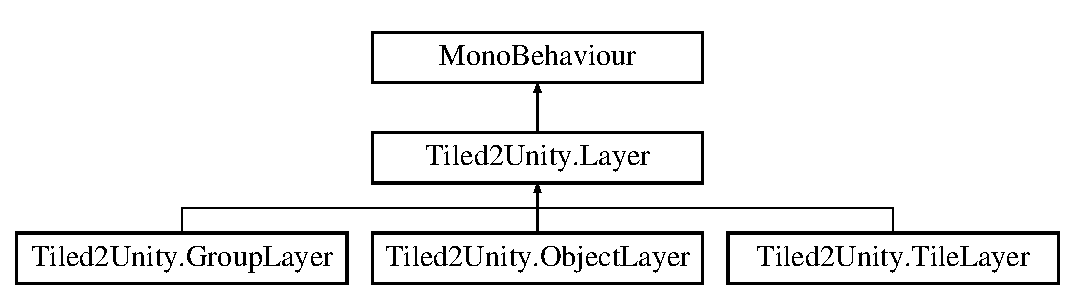
\includegraphics[height=3.000000cm]{class_tiled2_unity_1_1_layer}
\end{center}
\end{figure}
\subsection*{Public Attributes}
\begin{DoxyCompactItemize}
\item 
\mbox{\Hypertarget{class_tiled2_unity_1_1_layer_a59ea769705fb72a22ad0185d086001df}\label{class_tiled2_unity_1_1_layer_a59ea769705fb72a22ad0185d086001df}} 
Vector2 {\bfseries Offset}
\end{DoxyCompactItemize}


The documentation for this class was generated from the following file\+:\begin{DoxyCompactItemize}
\item 
Iso\+Chai/\+Assets/\+Tiled2\+Unity/\+Scripts/\+Runtime/Layer.\+cs\end{DoxyCompactItemize}

\hypertarget{class_tiled2_unity_1_1_logger}{}\section{Tiled2\+Unity.\+Logger Class Reference}
\label{class_tiled2_unity_1_1_logger}\index{Tiled2\+Unity.\+Logger@{Tiled2\+Unity.\+Logger}}
Inheritance diagram for Tiled2\+Unity.\+Logger\+:\begin{figure}[H]
\begin{center}
\leavevmode
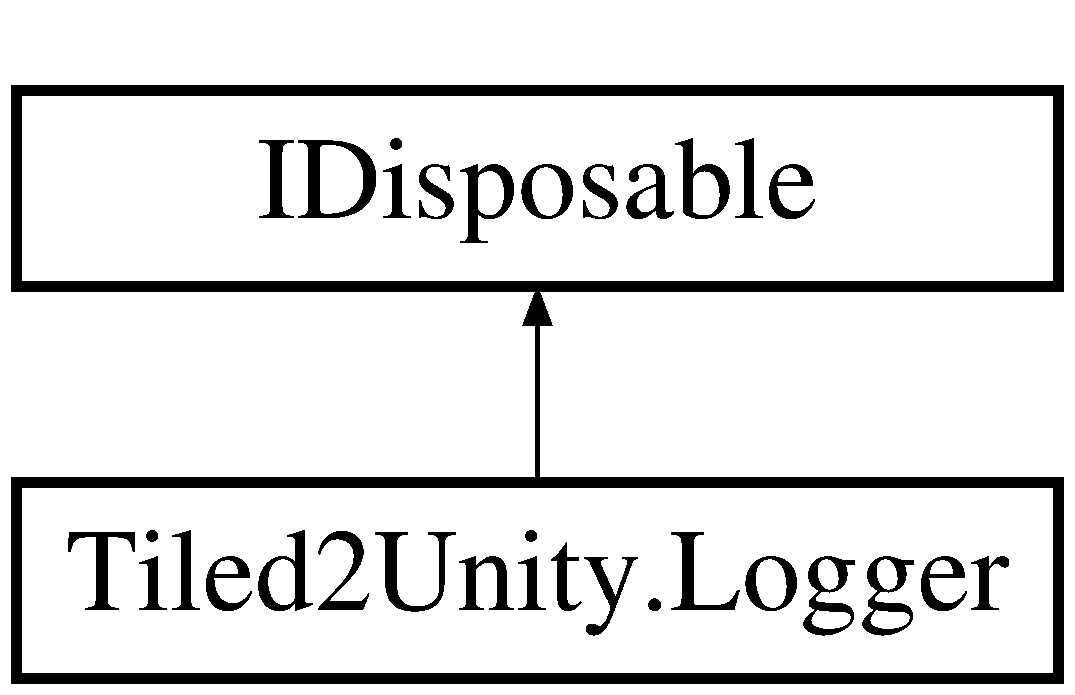
\includegraphics[height=2.000000cm]{class_tiled2_unity_1_1_logger}
\end{center}
\end{figure}
\subsection*{Public Member Functions}
\begin{DoxyCompactItemize}
\item 
\mbox{\Hypertarget{class_tiled2_unity_1_1_logger_aecf69e337c743c6e03298b97ef9bfb2d}\label{class_tiled2_unity_1_1_logger_aecf69e337c743c6e03298b97ef9bfb2d}} 
{\bfseries Logger} (string fmt, params object\mbox{[}$\,$\mbox{]} args)
\item 
\mbox{\Hypertarget{class_tiled2_unity_1_1_logger_a7531e7cdca3fd985d5c72be4d41d032a}\label{class_tiled2_unity_1_1_logger_a7531e7cdca3fd985d5c72be4d41d032a}} 
{\bfseries Logger} (string message)
\item 
\mbox{\Hypertarget{class_tiled2_unity_1_1_logger_ab5aa3518aaaa6bfb065bf5dc6a8a1e7e}\label{class_tiled2_unity_1_1_logger_ab5aa3518aaaa6bfb065bf5dc6a8a1e7e}} 
void {\bfseries Dispose} ()
\end{DoxyCompactItemize}


The documentation for this class was generated from the following file\+:\begin{DoxyCompactItemize}
\item 
Iso\+Chai/\+Assets/\+Tiled2\+Unity/\+Scripts/\+Runtime/Log.\+cs\end{DoxyCompactItemize}

\hypertarget{class_tiled2_unity_1_1_object_layer}{}\section{Tiled2\+Unity.\+Object\+Layer Class Reference}
\label{class_tiled2_unity_1_1_object_layer}\index{Tiled2\+Unity.\+Object\+Layer@{Tiled2\+Unity.\+Object\+Layer}}
Inheritance diagram for Tiled2\+Unity.\+Object\+Layer\+:\begin{figure}[H]
\begin{center}
\leavevmode
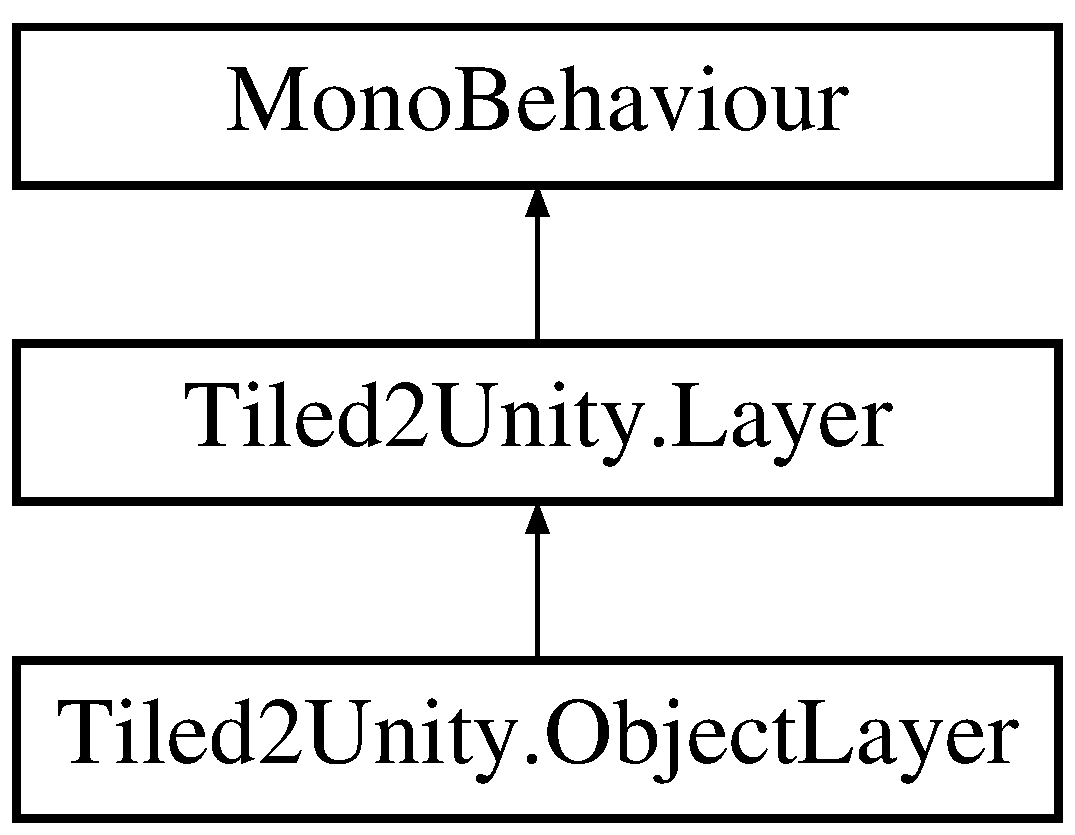
\includegraphics[height=3.000000cm]{class_tiled2_unity_1_1_object_layer}
\end{center}
\end{figure}
\subsection*{Public Attributes}
\begin{DoxyCompactItemize}
\item 
\mbox{\Hypertarget{class_tiled2_unity_1_1_object_layer_a4089059fb20eea72f30158d311868e54}\label{class_tiled2_unity_1_1_object_layer_a4089059fb20eea72f30158d311868e54}} 
Color {\bfseries Color}
\end{DoxyCompactItemize}


The documentation for this class was generated from the following file\+:\begin{DoxyCompactItemize}
\item 
Iso\+Chai/\+Assets/\+Tiled2\+Unity/\+Scripts/\+Runtime/Object\+Layer.\+cs\end{DoxyCompactItemize}

\hypertarget{class_tiled2_unity_1_1_polygon_object}{}\section{Tiled2\+Unity.\+Polygon\+Object Class Reference}
\label{class_tiled2_unity_1_1_polygon_object}\index{Tiled2\+Unity.\+Polygon\+Object@{Tiled2\+Unity.\+Polygon\+Object}}
Inheritance diagram for Tiled2\+Unity.\+Polygon\+Object\+:\begin{figure}[H]
\begin{center}
\leavevmode
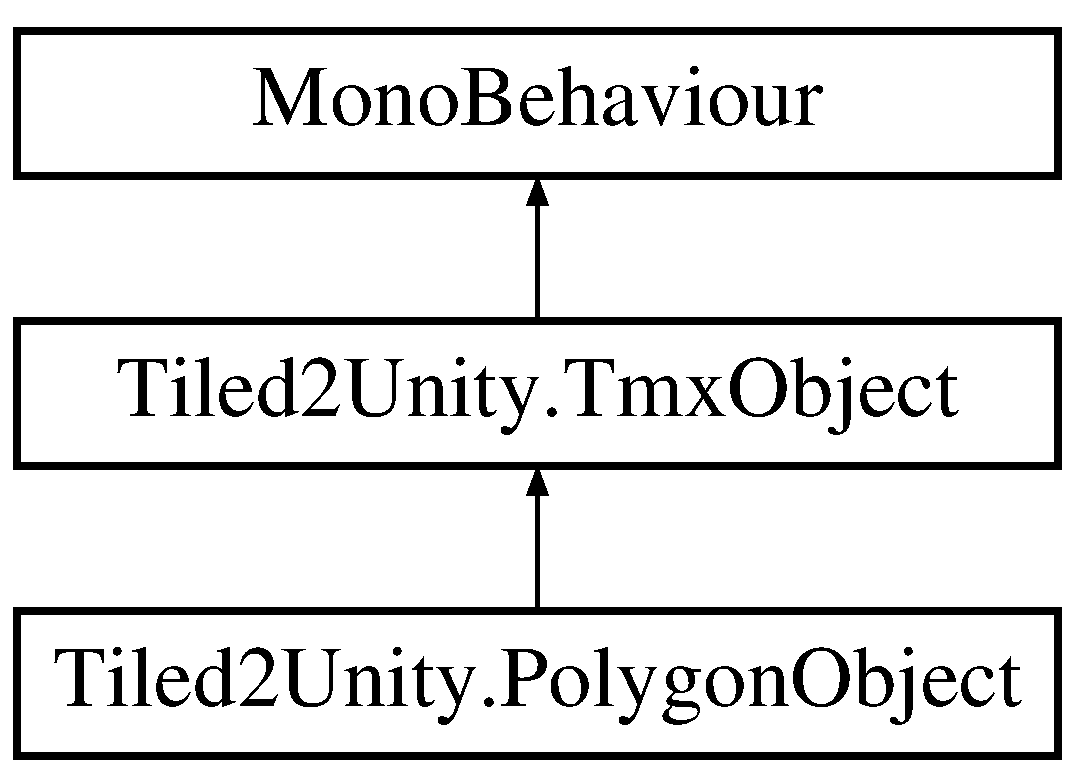
\includegraphics[height=3.000000cm]{class_tiled2_unity_1_1_polygon_object}
\end{center}
\end{figure}
\subsection*{Additional Inherited Members}


The documentation for this class was generated from the following file\+:\begin{DoxyCompactItemize}
\item 
D\+:/\+Users/\+Bennett/\+Desktop/\+School/\+E\+E\+C\+S\+\_\+448/\+Catch-\/the-\/\+Bus/\+Iso\+Chai/\+Assets/\+Tiled2\+Unity/\+Scripts/\+Runtime/Polygon\+Object.\+cs\end{DoxyCompactItemize}

\hypertarget{class_tiled2_unity_1_1_polyline_object}{}\section{Tiled2\+Unity.\+Polyline\+Object Class Reference}
\label{class_tiled2_unity_1_1_polyline_object}\index{Tiled2\+Unity.\+Polyline\+Object@{Tiled2\+Unity.\+Polyline\+Object}}
Inheritance diagram for Tiled2\+Unity.\+Polyline\+Object\+:\begin{figure}[H]
\begin{center}
\leavevmode
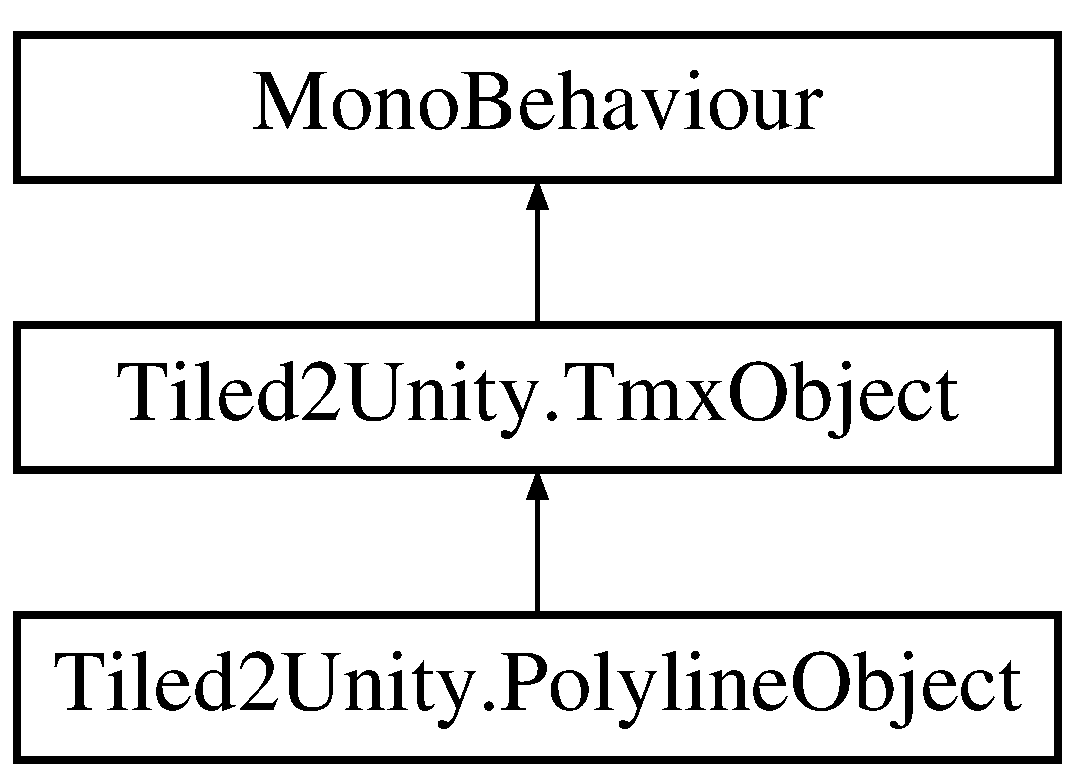
\includegraphics[height=3.000000cm]{class_tiled2_unity_1_1_polyline_object}
\end{center}
\end{figure}
\subsection*{Additional Inherited Members}


The documentation for this class was generated from the following file\+:\begin{DoxyCompactItemize}
\item 
D\+:/\+Users/\+Bennett/\+Desktop/\+School/\+E\+E\+C\+S\+\_\+448/\+Catch-\/the-\/\+Bus/\+Iso\+Chai/\+Assets/\+Tiled2\+Unity/\+Scripts/\+Runtime/Polyline\+Object.\+cs\end{DoxyCompactItemize}

\hypertarget{class_tiled2_unity_1_1_rectangle_object}{}\section{Tiled2\+Unity.\+Rectangle\+Object Class Reference}
\label{class_tiled2_unity_1_1_rectangle_object}\index{Tiled2\+Unity.\+Rectangle\+Object@{Tiled2\+Unity.\+Rectangle\+Object}}
Inheritance diagram for Tiled2\+Unity.\+Rectangle\+Object\+:\begin{figure}[H]
\begin{center}
\leavevmode
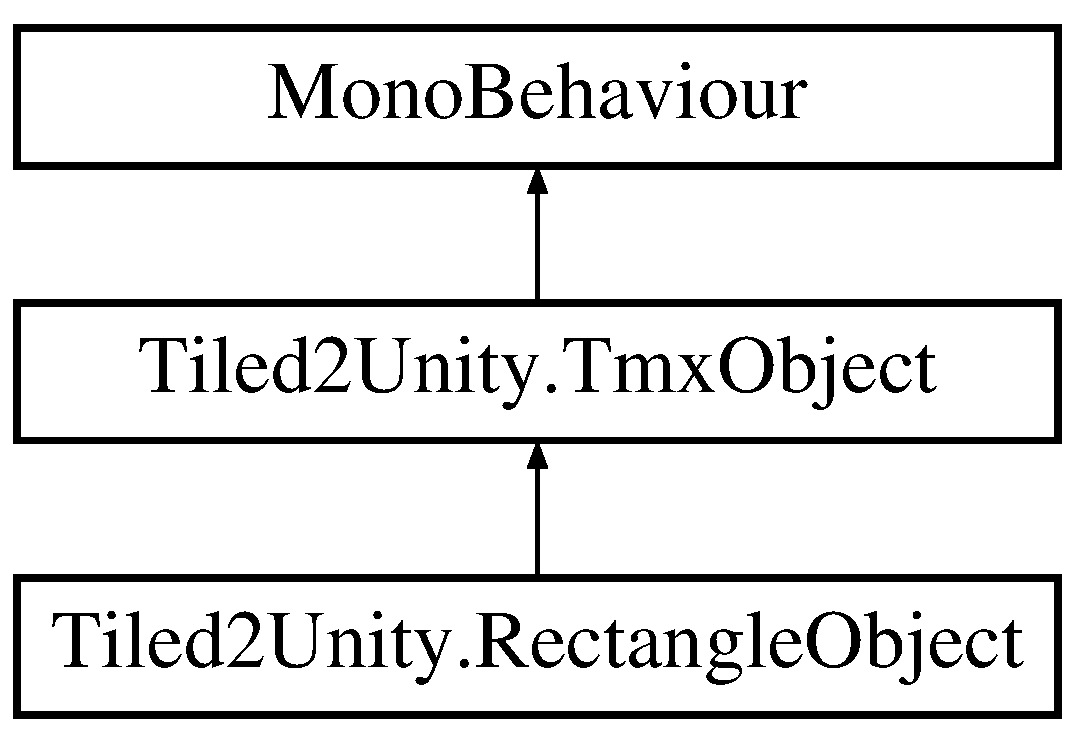
\includegraphics[height=3.000000cm]{class_tiled2_unity_1_1_rectangle_object}
\end{center}
\end{figure}
\subsection*{Additional Inherited Members}


The documentation for this class was generated from the following file\+:\begin{DoxyCompactItemize}
\item 
D\+:/\+Users/\+Bennett/\+Desktop/\+School/\+E\+E\+C\+S\+\_\+448/\+Catch-\/the-\/\+Bus/\+Iso\+Chai/\+Assets/\+Tiled2\+Unity/\+Scripts/\+Runtime/Rectangle\+Object.\+cs\end{DoxyCompactItemize}

\hypertarget{class_tiled2_unity_1_1_sorting_layer_exposed}{}\section{Tiled2\+Unity.\+Sorting\+Layer\+Exposed Class Reference}
\label{class_tiled2_unity_1_1_sorting_layer_exposed}\index{Tiled2\+Unity.\+Sorting\+Layer\+Exposed@{Tiled2\+Unity.\+Sorting\+Layer\+Exposed}}
Inheritance diagram for Tiled2\+Unity.\+Sorting\+Layer\+Exposed\+:\begin{figure}[H]
\begin{center}
\leavevmode
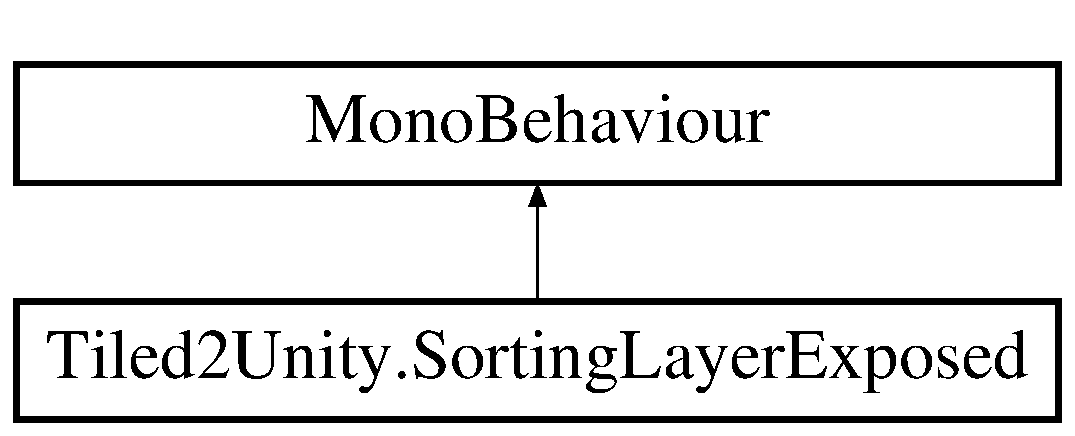
\includegraphics[height=2.000000cm]{class_tiled2_unity_1_1_sorting_layer_exposed}
\end{center}
\end{figure}


The documentation for this class was generated from the following file\+:\begin{DoxyCompactItemize}
\item 
Iso\+Chai/\+Assets/\+Tiled2\+Unity/\+Scripts/\+Runtime/Sorting\+Layer\+Exposed.\+cs\end{DoxyCompactItemize}

\hypertarget{class_sorting_layer_exposed_editor}{}\section{Sorting\+Layer\+Exposed\+Editor Class Reference}
\label{class_sorting_layer_exposed_editor}\index{Sorting\+Layer\+Exposed\+Editor@{Sorting\+Layer\+Exposed\+Editor}}
Inheritance diagram for Sorting\+Layer\+Exposed\+Editor\+:\begin{figure}[H]
\begin{center}
\leavevmode
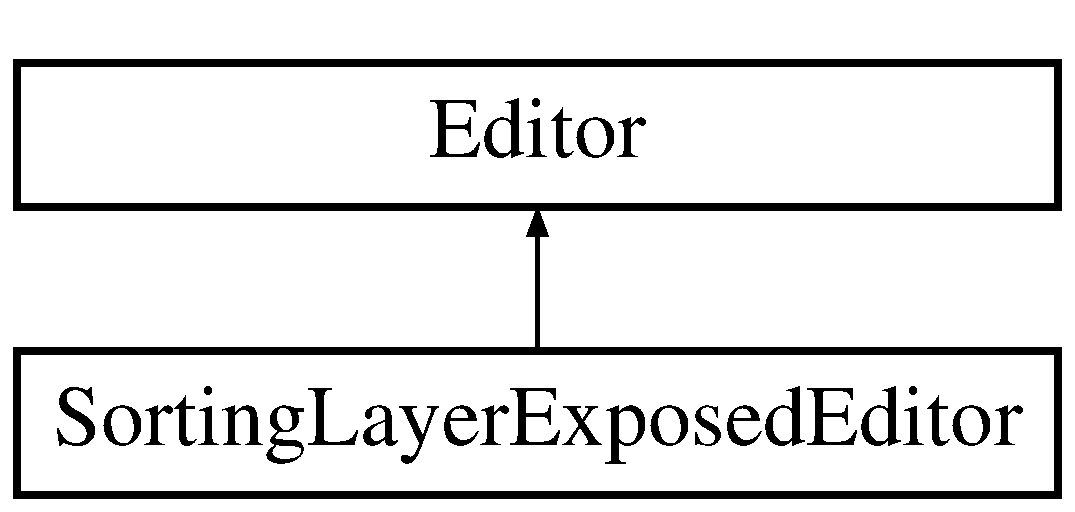
\includegraphics[height=2.000000cm]{class_sorting_layer_exposed_editor}
\end{center}
\end{figure}
\subsection*{Public Member Functions}
\begin{DoxyCompactItemize}
\item 
\mbox{\Hypertarget{class_sorting_layer_exposed_editor_a7ed0ea366de29a069582f71119303147}\label{class_sorting_layer_exposed_editor_a7ed0ea366de29a069582f71119303147}} 
override void {\bfseries On\+Inspector\+G\+UI} ()
\item 
\mbox{\Hypertarget{class_sorting_layer_exposed_editor_a34701bc7d634c91d10a5951c80634903}\label{class_sorting_layer_exposed_editor_a34701bc7d634c91d10a5951c80634903}} 
int \mbox{[}$\,$\mbox{]} {\bfseries Get\+Sorting\+Layer\+Unique\+I\+Ds} ()
\end{DoxyCompactItemize}
\subsection*{Static Public Member Functions}
\begin{DoxyCompactItemize}
\item 
\mbox{\Hypertarget{class_sorting_layer_exposed_editor_a3a80907acc6f4ebc060d072af00fda81}\label{class_sorting_layer_exposed_editor_a3a80907acc6f4ebc060d072af00fda81}} 
static G\+U\+I\+Content \mbox{[}$\,$\mbox{]} {\bfseries Get\+Sorting\+Layer\+Contexts} ()
\item 
\mbox{\Hypertarget{class_sorting_layer_exposed_editor_a5fe8e0af24db48e01353b98ed02a3768}\label{class_sorting_layer_exposed_editor_a5fe8e0af24db48e01353b98ed02a3768}} 
static string \mbox{[}$\,$\mbox{]} {\bfseries Get\+Sorting\+Layer\+Names} ()
\item 
\mbox{\Hypertarget{class_sorting_layer_exposed_editor_afbc49b8a12d797616c8afda74ed86aac}\label{class_sorting_layer_exposed_editor_afbc49b8a12d797616c8afda74ed86aac}} 
static int {\bfseries Get\+Sorting\+Layer\+Index} (Renderer renderer, string\mbox{[}$\,$\mbox{]} layer\+Names)
\item 
\mbox{\Hypertarget{class_sorting_layer_exposed_editor_a9d280defdaf4d581d17333c339e3e76a}\label{class_sorting_layer_exposed_editor_a9d280defdaf4d581d17333c339e3e76a}} 
static int {\bfseries Get\+Sorting\+Layer\+Id\+Index} (Renderer renderer, int\mbox{[}$\,$\mbox{]} layer\+Ids)
\end{DoxyCompactItemize}


The documentation for this class was generated from the following file\+:\begin{DoxyCompactItemize}
\item 
Iso\+Chai/\+Assets/\+Tiled2\+Unity/\+Scripts/\+Editor/Sorting\+Layer\+Exposed\+Editor.\+cs\end{DoxyCompactItemize}

\hypertarget{class_tiled2_unity_1_1_sprite_depth_in_map}{}\section{Tiled2\+Unity.\+Sprite\+Depth\+In\+Map Class Reference}
\label{class_tiled2_unity_1_1_sprite_depth_in_map}\index{Tiled2\+Unity.\+Sprite\+Depth\+In\+Map@{Tiled2\+Unity.\+Sprite\+Depth\+In\+Map}}
Inheritance diagram for Tiled2\+Unity.\+Sprite\+Depth\+In\+Map\+:\begin{figure}[H]
\begin{center}
\leavevmode
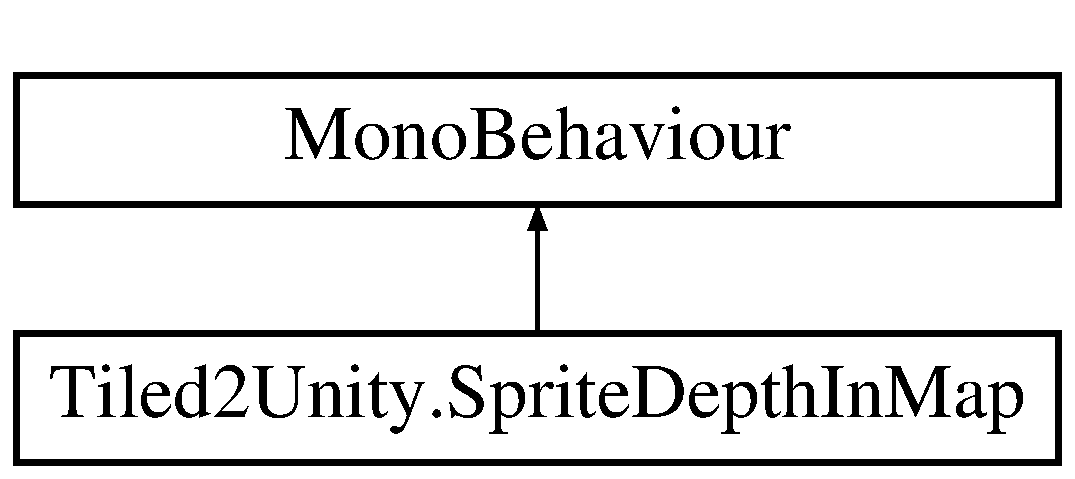
\includegraphics[height=2.000000cm]{class_tiled2_unity_1_1_sprite_depth_in_map}
\end{center}
\end{figure}
\subsection*{Public Member Functions}
\begin{DoxyCompactItemize}
\item 
\mbox{\Hypertarget{class_tiled2_unity_1_1_sprite_depth_in_map_a79ca9fab2c970a7b1b38ac517b1b7e4f}\label{class_tiled2_unity_1_1_sprite_depth_in_map_a79ca9fab2c970a7b1b38ac517b1b7e4f}} 
void {\bfseries Update\+Sprite\+Depth} ()
\end{DoxyCompactItemize}
\subsection*{Public Attributes}
\begin{DoxyCompactItemize}
\item 
\mbox{\Hypertarget{class_tiled2_unity_1_1_sprite_depth_in_map_a5dd8f08b23b777e39c8b487c83f031d5}\label{class_tiled2_unity_1_1_sprite_depth_in_map_a5dd8f08b23b777e39c8b487c83f031d5}} 
\mbox{\hyperlink{class_tiled2_unity_1_1_tiled_map}{Tiled2\+Unity.\+Tiled\+Map}} {\bfseries Attached\+Map} = null
\item 
\mbox{\Hypertarget{class_tiled2_unity_1_1_sprite_depth_in_map_aa4341e388711f701a946f7cbd28ca0ca}\label{class_tiled2_unity_1_1_sprite_depth_in_map_aa4341e388711f701a946f7cbd28ca0ca}} 
int {\bfseries Interact\+With\+Layer} = 0
\item 
\mbox{\Hypertarget{class_tiled2_unity_1_1_sprite_depth_in_map_a0f4e0cf735c9ec63f3362751b89edd60}\label{class_tiled2_unity_1_1_sprite_depth_in_map_a0f4e0cf735c9ec63f3362751b89edd60}} 
int {\bfseries Tileset\+Height} = 0
\end{DoxyCompactItemize}


The documentation for this class was generated from the following file\+:\begin{DoxyCompactItemize}
\item 
D\+:/\+Users/\+Bennett/\+Desktop/\+School/\+E\+E\+C\+S\+\_\+448/\+Catch-\/the-\/\+Bus/\+Iso\+Chai/\+Assets/\+Tiled2\+Unity/\+Scripts/\+Runtime/Sprite\+Depth\+In\+Map.\+cs\end{DoxyCompactItemize}

\hypertarget{class_tiled2_unity_1_1_sprite_depth_in_map_editor}{}\section{Tiled2\+Unity.\+Sprite\+Depth\+In\+Map\+Editor Class Reference}
\label{class_tiled2_unity_1_1_sprite_depth_in_map_editor}\index{Tiled2\+Unity.\+Sprite\+Depth\+In\+Map\+Editor@{Tiled2\+Unity.\+Sprite\+Depth\+In\+Map\+Editor}}
Inheritance diagram for Tiled2\+Unity.\+Sprite\+Depth\+In\+Map\+Editor\+:\begin{figure}[H]
\begin{center}
\leavevmode
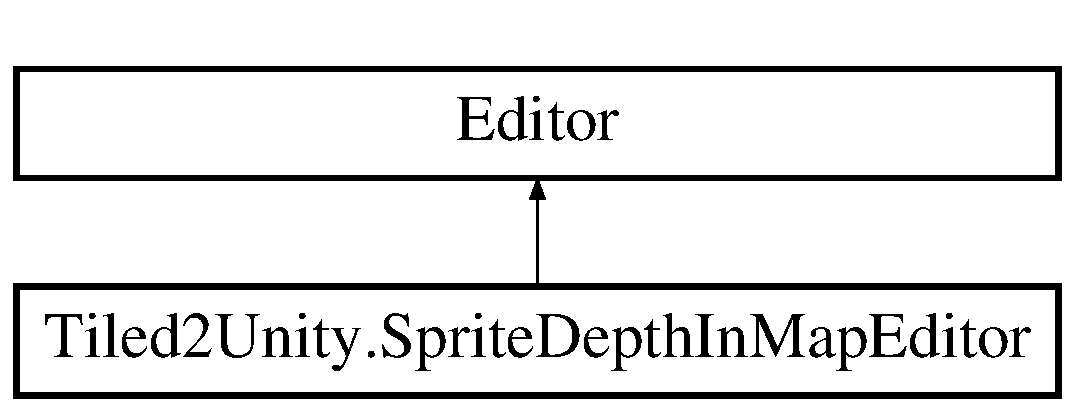
\includegraphics[height=2.000000cm]{class_tiled2_unity_1_1_sprite_depth_in_map_editor}
\end{center}
\end{figure}
\subsection*{Public Member Functions}
\begin{DoxyCompactItemize}
\item 
\mbox{\Hypertarget{class_tiled2_unity_1_1_sprite_depth_in_map_editor_aa56bfe7c8ed00dbe8ce3e20f52cd17c6}\label{class_tiled2_unity_1_1_sprite_depth_in_map_editor_aa56bfe7c8ed00dbe8ce3e20f52cd17c6}} 
override void {\bfseries On\+Inspector\+G\+UI} ()
\end{DoxyCompactItemize}


The documentation for this class was generated from the following file\+:\begin{DoxyCompactItemize}
\item 
D\+:/\+Users/\+Bennett/\+Desktop/\+School/\+E\+E\+C\+S\+\_\+448/\+Catch-\/the-\/\+Bus/\+Iso\+Chai/\+Assets/\+Tiled2\+Unity/\+Scripts/\+Editor/Sprite\+Depth\+In\+Map\+Editor.\+cs\end{DoxyCompactItemize}

\hypertarget{class_tiled2_unity_1_1_tile_animator}{}\section{Tiled2\+Unity.\+Tile\+Animator Class Reference}
\label{class_tiled2_unity_1_1_tile_animator}\index{Tiled2\+Unity.\+Tile\+Animator@{Tiled2\+Unity.\+Tile\+Animator}}
Inheritance diagram for Tiled2\+Unity.\+Tile\+Animator\+:\begin{figure}[H]
\begin{center}
\leavevmode
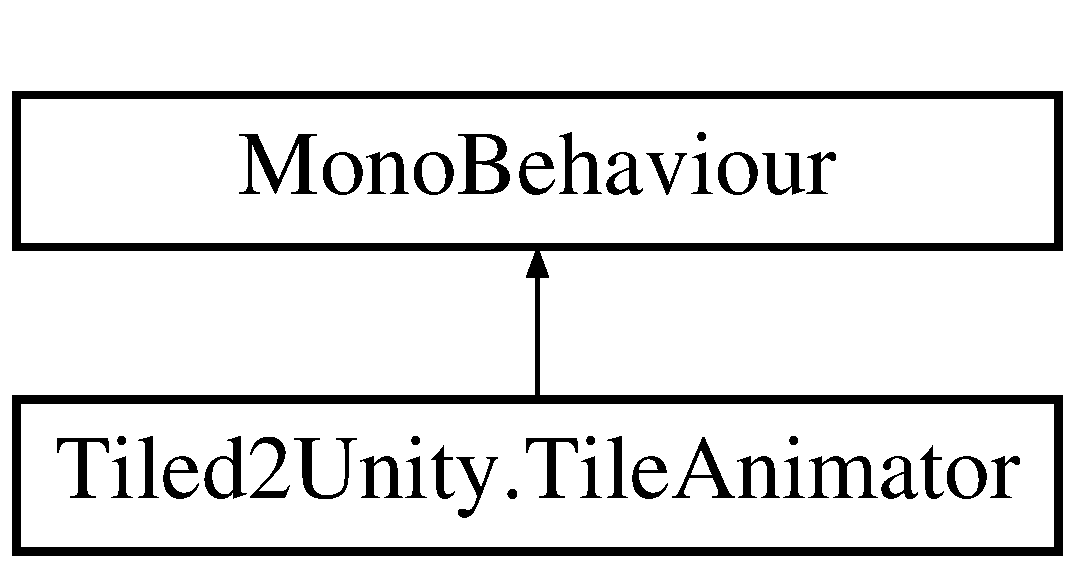
\includegraphics[height=2.000000cm]{class_tiled2_unity_1_1_tile_animator}
\end{center}
\end{figure}
\subsection*{Public Attributes}
\begin{DoxyCompactItemize}
\item 
\mbox{\Hypertarget{class_tiled2_unity_1_1_tile_animator_ac96cabb3b772e367d4141dba085a459b}\label{class_tiled2_unity_1_1_tile_animator_ac96cabb3b772e367d4141dba085a459b}} 
float {\bfseries Start\+Time} = -\/1
\item 
\mbox{\Hypertarget{class_tiled2_unity_1_1_tile_animator_a36a9be6b0075d46cd283eba6ed110f02}\label{class_tiled2_unity_1_1_tile_animator_a36a9be6b0075d46cd283eba6ed110f02}} 
float {\bfseries Duration} = -\/1
\item 
\mbox{\Hypertarget{class_tiled2_unity_1_1_tile_animator_abfc3c29538506faf9f4f8ef8bd438839}\label{class_tiled2_unity_1_1_tile_animator_abfc3c29538506faf9f4f8ef8bd438839}} 
float {\bfseries Total\+Animation\+Time} = -\/1
\end{DoxyCompactItemize}


The documentation for this class was generated from the following file\+:\begin{DoxyCompactItemize}
\item 
D\+:/\+Users/\+Bennett/\+Desktop/\+School/\+E\+E\+C\+S\+\_\+448/\+Catch-\/the-\/\+Bus/\+Iso\+Chai/\+Assets/\+Tiled2\+Unity/\+Scripts/\+Runtime/Tile\+Animator.\+cs\end{DoxyCompactItemize}

\hypertarget{class_tiled2_unity_1_1_tiled2_unity_menu_items}{}\section{Tiled2\+Unity.\+Tiled2\+Unity\+Menu\+Items Class Reference}
\label{class_tiled2_unity_1_1_tiled2_unity_menu_items}\index{Tiled2\+Unity.\+Tiled2\+Unity\+Menu\+Items@{Tiled2\+Unity.\+Tiled2\+Unity\+Menu\+Items}}


The documentation for this class was generated from the following file\+:\begin{DoxyCompactItemize}
\item 
D\+:/\+Users/\+Bennett/\+Desktop/\+School/\+E\+E\+C\+S\+\_\+448/\+Catch-\/the-\/\+Bus/\+Iso\+Chai/\+Assets/\+Tiled2\+Unity/\+Scripts/\+Editor/Tiled2\+Unity\+Menu\+Items.\+cs\end{DoxyCompactItemize}

\hypertarget{class_tiled2_unity_1_1_tiled_asset_post_processor}{}\section{Tiled2\+Unity.\+Tiled\+Asset\+Post\+Processor Class Reference}
\label{class_tiled2_unity_1_1_tiled_asset_post_processor}\index{Tiled2\+Unity.\+Tiled\+Asset\+Post\+Processor@{Tiled2\+Unity.\+Tiled\+Asset\+Post\+Processor}}
Inheritance diagram for Tiled2\+Unity.\+Tiled\+Asset\+Post\+Processor\+:\begin{figure}[H]
\begin{center}
\leavevmode
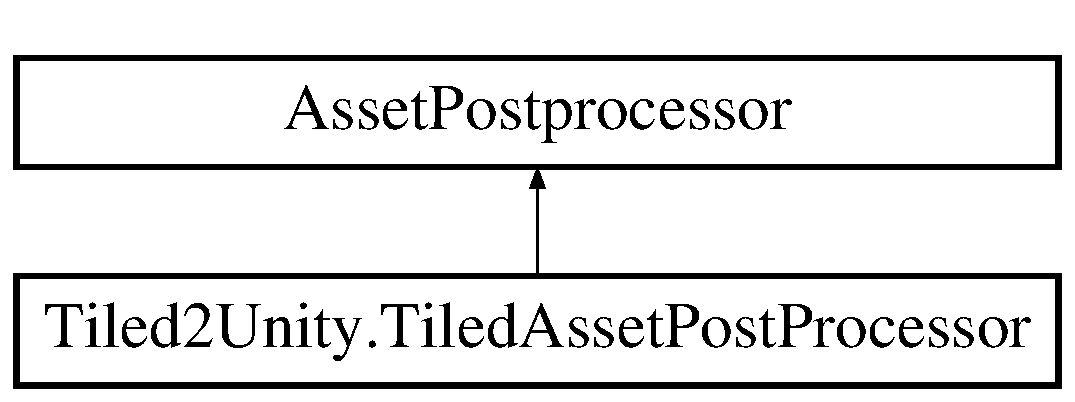
\includegraphics[height=2.000000cm]{class_tiled2_unity_1_1_tiled_asset_post_processor}
\end{center}
\end{figure}


The documentation for this class was generated from the following file\+:\begin{DoxyCompactItemize}
\item 
Iso\+Chai/\+Assets/\+Tiled2\+Unity/\+Scripts/\+Editor/Tiled\+Asset\+Post\+Processor.\+cs\end{DoxyCompactItemize}

\hypertarget{class_tiled2_unity_1_1_tiled_map}{}\section{Tiled2\+Unity.\+Tiled\+Map Class Reference}
\label{class_tiled2_unity_1_1_tiled_map}\index{Tiled2\+Unity.\+Tiled\+Map@{Tiled2\+Unity.\+Tiled\+Map}}
Inheritance diagram for Tiled2\+Unity.\+Tiled\+Map\+:\begin{figure}[H]
\begin{center}
\leavevmode
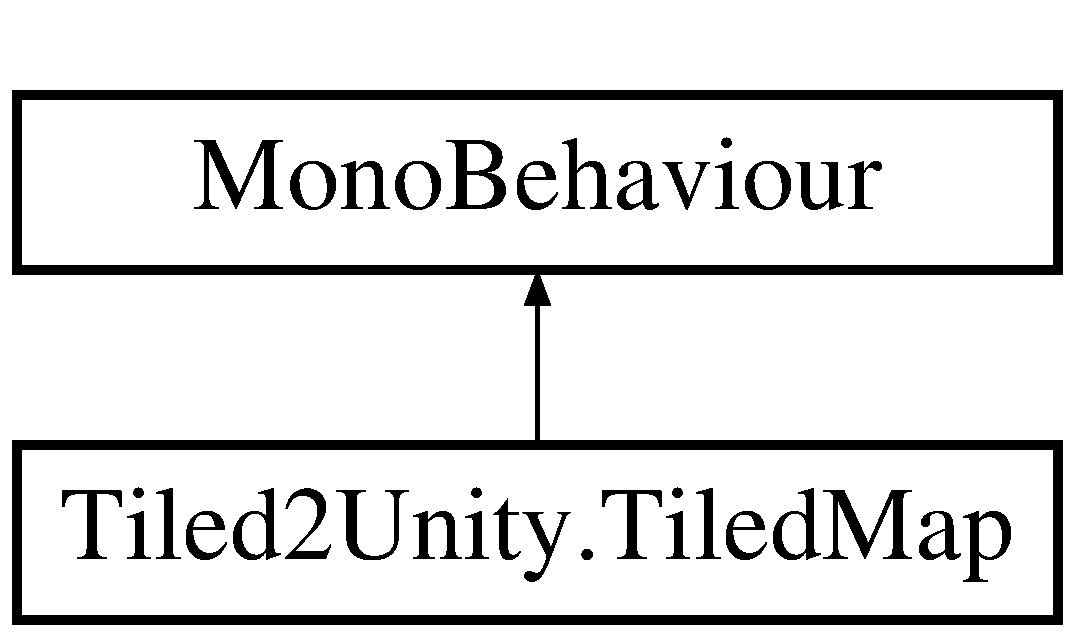
\includegraphics[height=2.000000cm]{class_tiled2_unity_1_1_tiled_map}
\end{center}
\end{figure}
\subsection*{Public Types}
\begin{DoxyCompactItemize}
\item 
\mbox{\Hypertarget{class_tiled2_unity_1_1_tiled_map_a10fd626f5ab8d58e41c50d30829d28c3}\label{class_tiled2_unity_1_1_tiled_map_a10fd626f5ab8d58e41c50d30829d28c3}} 
enum {\bfseries Map\+Orientation} \{ {\bfseries Orthogonal}, 
{\bfseries Isometric}, 
{\bfseries Staggered}, 
{\bfseries Hexagonal}
 \}
\item 
\mbox{\Hypertarget{class_tiled2_unity_1_1_tiled_map_ad518b3edd3ec47ca251249cb096c0a8d}\label{class_tiled2_unity_1_1_tiled_map_ad518b3edd3ec47ca251249cb096c0a8d}} 
enum {\bfseries Map\+Stagger\+Axis} \{ {\bfseries X}, 
{\bfseries Y}
 \}
\item 
\mbox{\Hypertarget{class_tiled2_unity_1_1_tiled_map_a18de2ab433a61d0e6e40117e0a2f0fd7}\label{class_tiled2_unity_1_1_tiled_map_a18de2ab433a61d0e6e40117e0a2f0fd7}} 
enum {\bfseries Map\+Stagger\+Index} \{ {\bfseries Odd}, 
{\bfseries Even}
 \}
\end{DoxyCompactItemize}
\subsection*{Public Member Functions}
\begin{DoxyCompactItemize}
\item 
\mbox{\Hypertarget{class_tiled2_unity_1_1_tiled_map_ad78f1e4e5bb593c9f6e2475694699551}\label{class_tiled2_unity_1_1_tiled_map_ad78f1e4e5bb593c9f6e2475694699551}} 
float {\bfseries Get\+Map\+Width\+In\+Pixels\+Scaled} ()
\item 
\mbox{\Hypertarget{class_tiled2_unity_1_1_tiled_map_adefe738f0c07edfbd65bf4f08cb85a2e}\label{class_tiled2_unity_1_1_tiled_map_adefe738f0c07edfbd65bf4f08cb85a2e}} 
float {\bfseries Get\+Map\+Height\+In\+Pixels\+Scaled} ()
\item 
\mbox{\Hypertarget{class_tiled2_unity_1_1_tiled_map_aba80a33188bdec8817437d139ab38a28}\label{class_tiled2_unity_1_1_tiled_map_aba80a33188bdec8817437d139ab38a28}} 
Rect {\bfseries Get\+Map\+Rect} ()
\item 
\mbox{\Hypertarget{class_tiled2_unity_1_1_tiled_map_a3c2a17fcdb0e1dd442c2b65ba90ba929}\label{class_tiled2_unity_1_1_tiled_map_a3c2a17fcdb0e1dd442c2b65ba90ba929}} 
Rect {\bfseries Get\+Map\+Rect\+In\+Pixels\+Scaled} ()
\item 
\mbox{\Hypertarget{class_tiled2_unity_1_1_tiled_map_a75f0eef03671de5ec3417e9404f1a050}\label{class_tiled2_unity_1_1_tiled_map_a75f0eef03671de5ec3417e9404f1a050}} 
bool {\bfseries Are\+Tiles\+Staggered} ()
\end{DoxyCompactItemize}
\subsection*{Public Attributes}
\begin{DoxyCompactItemize}
\item 
\mbox{\Hypertarget{class_tiled2_unity_1_1_tiled_map_a82a481deedf123c6ce6c9c6fc171cb12}\label{class_tiled2_unity_1_1_tiled_map_a82a481deedf123c6ce6c9c6fc171cb12}} 
Map\+Orientation {\bfseries Orientation} = Map\+Orientation.\+Orthogonal
\item 
\mbox{\Hypertarget{class_tiled2_unity_1_1_tiled_map_a09b071640cf98506103a5f08c296ab39}\label{class_tiled2_unity_1_1_tiled_map_a09b071640cf98506103a5f08c296ab39}} 
Map\+Stagger\+Axis {\bfseries Stagger\+Axis} = Map\+Stagger\+Axis.\+X
\item 
\mbox{\Hypertarget{class_tiled2_unity_1_1_tiled_map_a808ab5ae9df00c2c93e14459f021c944}\label{class_tiled2_unity_1_1_tiled_map_a808ab5ae9df00c2c93e14459f021c944}} 
Map\+Stagger\+Index {\bfseries Stagger\+Index} = Map\+Stagger\+Index.\+Odd
\item 
\mbox{\Hypertarget{class_tiled2_unity_1_1_tiled_map_a4a8a2c09936e8741dea8aa07c809b469}\label{class_tiled2_unity_1_1_tiled_map_a4a8a2c09936e8741dea8aa07c809b469}} 
int {\bfseries Hex\+Side\+Length} = 0
\item 
\mbox{\Hypertarget{class_tiled2_unity_1_1_tiled_map_a806b2071a7144933a803a23e15810e21}\label{class_tiled2_unity_1_1_tiled_map_a806b2071a7144933a803a23e15810e21}} 
int {\bfseries Num\+Layers} = 0
\item 
\mbox{\Hypertarget{class_tiled2_unity_1_1_tiled_map_a4751f960675fce0b710bfeb8a364278c}\label{class_tiled2_unity_1_1_tiled_map_a4751f960675fce0b710bfeb8a364278c}} 
int {\bfseries Num\+Tiles\+Wide} = 0
\item 
\mbox{\Hypertarget{class_tiled2_unity_1_1_tiled_map_afb22dd4537a08cf3325bf5eafe0d14d1}\label{class_tiled2_unity_1_1_tiled_map_afb22dd4537a08cf3325bf5eafe0d14d1}} 
int {\bfseries Num\+Tiles\+High} = 0
\item 
\mbox{\Hypertarget{class_tiled2_unity_1_1_tiled_map_a41427ef6894ce19eed5d5fc3429eb9e0}\label{class_tiled2_unity_1_1_tiled_map_a41427ef6894ce19eed5d5fc3429eb9e0}} 
int {\bfseries Tile\+Width} = 0
\item 
\mbox{\Hypertarget{class_tiled2_unity_1_1_tiled_map_a4efa3016fa647fbef3ad703377b00e13}\label{class_tiled2_unity_1_1_tiled_map_a4efa3016fa647fbef3ad703377b00e13}} 
int {\bfseries Tile\+Height} = 0
\item 
\mbox{\Hypertarget{class_tiled2_unity_1_1_tiled_map_a608dfffdbb33b68d4f810e4e0c1e97c4}\label{class_tiled2_unity_1_1_tiled_map_a608dfffdbb33b68d4f810e4e0c1e97c4}} 
float {\bfseries Export\+Scale} = 1.\+0f
\item 
\mbox{\Hypertarget{class_tiled2_unity_1_1_tiled_map_aa494770e2f38b482a4adee6990e687ab}\label{class_tiled2_unity_1_1_tiled_map_aa494770e2f38b482a4adee6990e687ab}} 
int {\bfseries Map\+Width\+In\+Pixels} = 0
\item 
\mbox{\Hypertarget{class_tiled2_unity_1_1_tiled_map_a6a10e2ec0f364481ae2268ab8bb40941}\label{class_tiled2_unity_1_1_tiled_map_a6a10e2ec0f364481ae2268ab8bb40941}} 
int {\bfseries Map\+Height\+In\+Pixels} = 0
\item 
\mbox{\Hypertarget{class_tiled2_unity_1_1_tiled_map_aa3ec5f9703ec523511b17561fa736eda}\label{class_tiled2_unity_1_1_tiled_map_aa3ec5f9703ec523511b17561fa736eda}} 
Color {\bfseries Background\+Color} = Color.\+black
\end{DoxyCompactItemize}


The documentation for this class was generated from the following file\+:\begin{DoxyCompactItemize}
\item 
D\+:/\+Users/\+Bennett/\+Desktop/\+School/\+E\+E\+C\+S\+\_\+448/\+Catch-\/the-\/\+Bus/\+Iso\+Chai/\+Assets/\+Tiled2\+Unity/\+Scripts/\+Runtime/Tiled\+Map.\+cs\end{DoxyCompactItemize}

\hypertarget{class_tiled2_unity_1_1_tile_layer}{}\section{Tiled2\+Unity.\+Tile\+Layer Class Reference}
\label{class_tiled2_unity_1_1_tile_layer}\index{Tiled2\+Unity.\+Tile\+Layer@{Tiled2\+Unity.\+Tile\+Layer}}
Inheritance diagram for Tiled2\+Unity.\+Tile\+Layer\+:\begin{figure}[H]
\begin{center}
\leavevmode
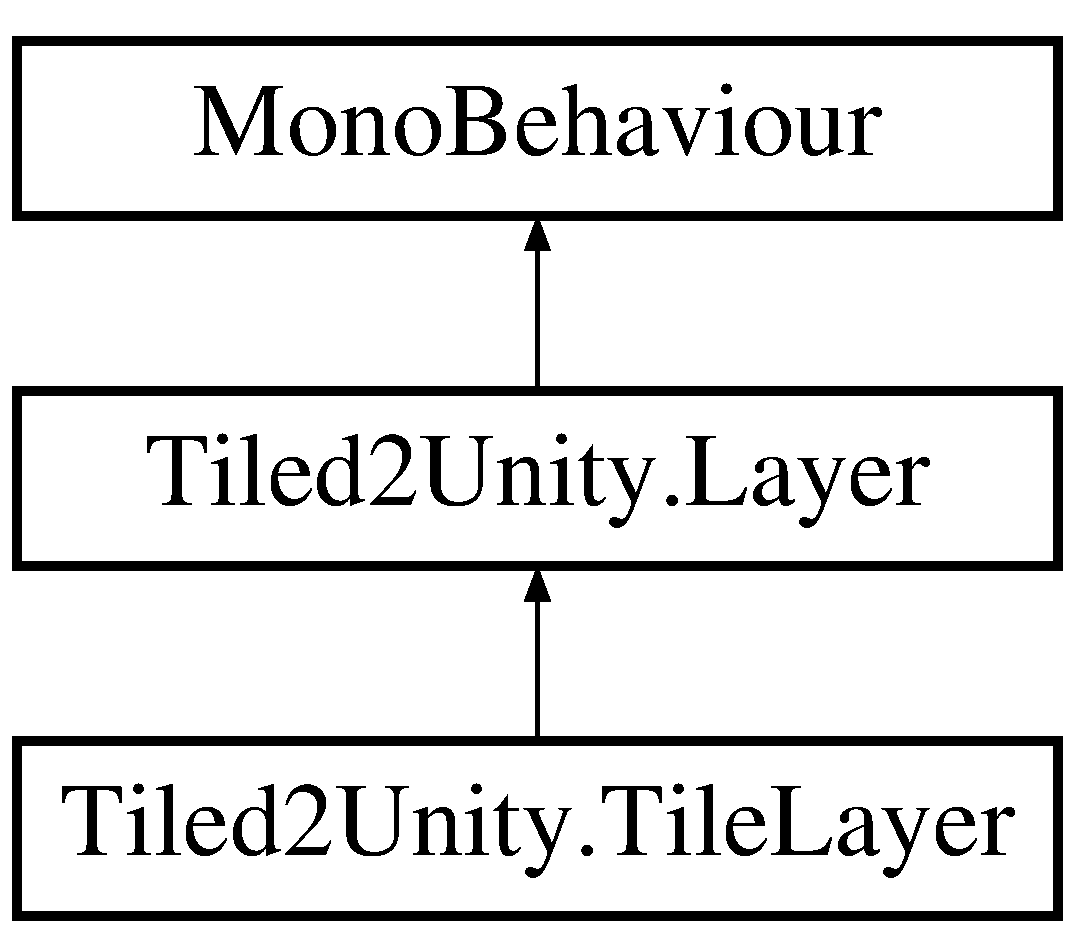
\includegraphics[height=3.000000cm]{class_tiled2_unity_1_1_tile_layer}
\end{center}
\end{figure}
\subsection*{Additional Inherited Members}


The documentation for this class was generated from the following file\+:\begin{DoxyCompactItemize}
\item 
D\+:/\+Users/\+Bennett/\+Desktop/\+School/\+E\+E\+C\+S\+\_\+448/\+Catch-\/the-\/\+Bus/\+Iso\+Chai/\+Assets/\+Tiled2\+Unity/\+Scripts/\+Runtime/Tile\+Layer.\+cs\end{DoxyCompactItemize}

\hypertarget{class_tiled2_unity_1_1_tile_object}{}\section{Tiled2\+Unity.\+Tile\+Object Class Reference}
\label{class_tiled2_unity_1_1_tile_object}\index{Tiled2\+Unity.\+Tile\+Object@{Tiled2\+Unity.\+Tile\+Object}}
Inheritance diagram for Tiled2\+Unity.\+Tile\+Object\+:\begin{figure}[H]
\begin{center}
\leavevmode
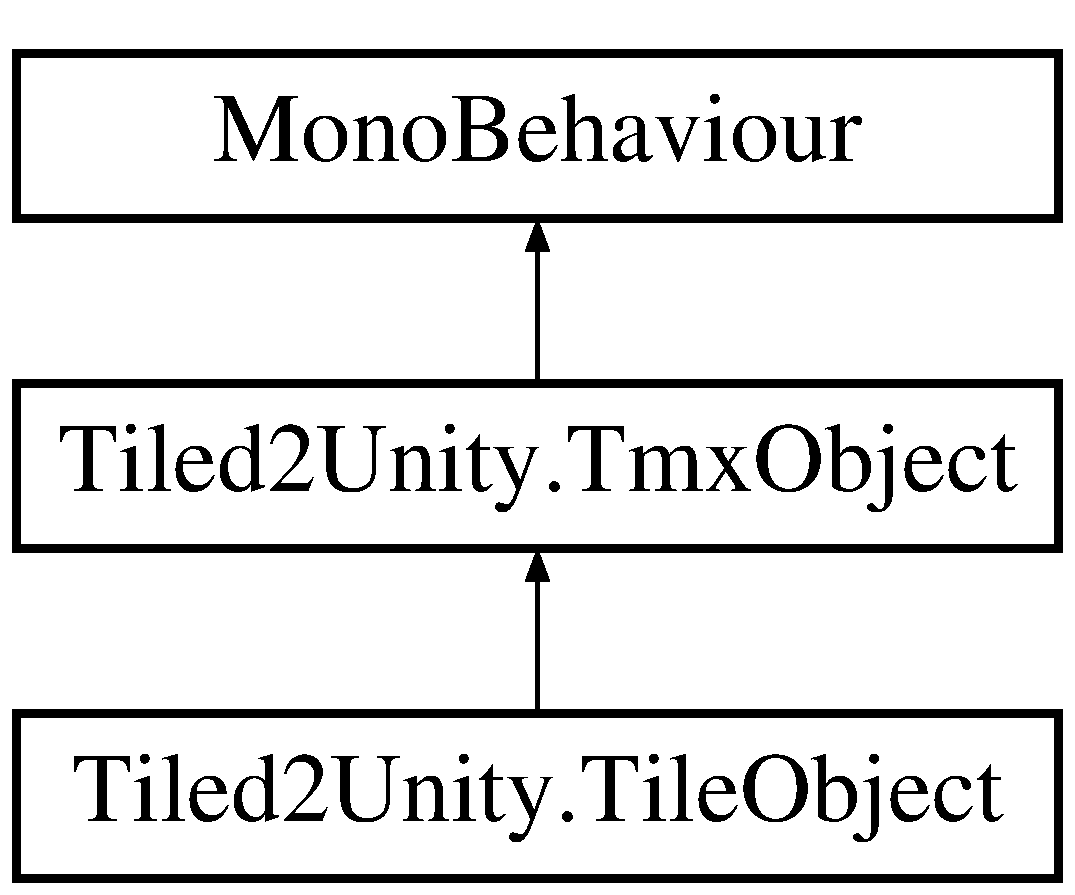
\includegraphics[height=3.000000cm]{class_tiled2_unity_1_1_tile_object}
\end{center}
\end{figure}
\subsection*{Public Attributes}
\begin{DoxyCompactItemize}
\item 
\mbox{\Hypertarget{class_tiled2_unity_1_1_tile_object_abafd4afef3f59c65ca1bc370ce1af9f7}\label{class_tiled2_unity_1_1_tile_object_abafd4afef3f59c65ca1bc370ce1af9f7}} 
bool {\bfseries Tmx\+Flipping\+Horizontal}
\item 
\mbox{\Hypertarget{class_tiled2_unity_1_1_tile_object_a90fdfe12d49c2e7bc900d3ad73a5f0da}\label{class_tiled2_unity_1_1_tile_object_a90fdfe12d49c2e7bc900d3ad73a5f0da}} 
bool {\bfseries Tmx\+Flipping\+Vertical}
\item 
\mbox{\Hypertarget{class_tiled2_unity_1_1_tile_object_af124dfbce4dee89e7d41ab53fc7a3a23}\label{class_tiled2_unity_1_1_tile_object_af124dfbce4dee89e7d41ab53fc7a3a23}} 
float {\bfseries Tile\+Width} = 0.\+0f
\item 
\mbox{\Hypertarget{class_tiled2_unity_1_1_tile_object_a03f3f899c6efc1fa8f79f377fcfa12bd}\label{class_tiled2_unity_1_1_tile_object_a03f3f899c6efc1fa8f79f377fcfa12bd}} 
float {\bfseries Tile\+Height} = 0.\+0f
\end{DoxyCompactItemize}


The documentation for this class was generated from the following file\+:\begin{DoxyCompactItemize}
\item 
D\+:/\+Users/\+Bennett/\+Desktop/\+School/\+E\+E\+C\+S\+\_\+448/\+Catch-\/the-\/\+Bus/\+Iso\+Chai/\+Assets/\+Tiled2\+Unity/\+Scripts/\+Runtime/Tile\+Object.\+cs\end{DoxyCompactItemize}

\hypertarget{class_tiled2_unity_1_1_tmx_object}{}\section{Tiled2\+Unity.\+Tmx\+Object Class Reference}
\label{class_tiled2_unity_1_1_tmx_object}\index{Tiled2\+Unity.\+Tmx\+Object@{Tiled2\+Unity.\+Tmx\+Object}}
Inheritance diagram for Tiled2\+Unity.\+Tmx\+Object\+:\begin{figure}[H]
\begin{center}
\leavevmode
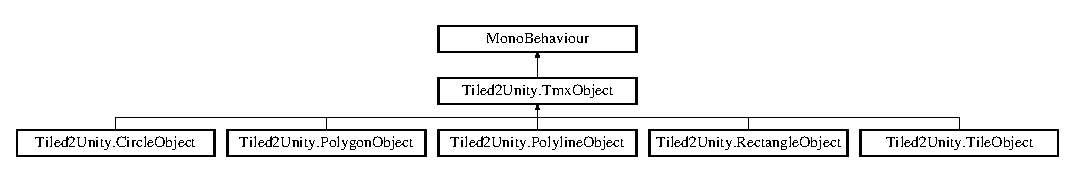
\includegraphics[height=1.877095cm]{class_tiled2_unity_1_1_tmx_object}
\end{center}
\end{figure}
\subsection*{Public Attributes}
\begin{DoxyCompactItemize}
\item 
\mbox{\Hypertarget{class_tiled2_unity_1_1_tmx_object_af523fddb695142cbb86c0eaca115e883}\label{class_tiled2_unity_1_1_tmx_object_af523fddb695142cbb86c0eaca115e883}} 
int {\bfseries Tmx\+Id}
\item 
\mbox{\Hypertarget{class_tiled2_unity_1_1_tmx_object_a865abf541cffb969b3650374a07acb64}\label{class_tiled2_unity_1_1_tmx_object_a865abf541cffb969b3650374a07acb64}} 
string {\bfseries Tmx\+Name}
\item 
\mbox{\Hypertarget{class_tiled2_unity_1_1_tmx_object_a1ebc9e3f4e1678dcf293df85e8412c1d}\label{class_tiled2_unity_1_1_tmx_object_a1ebc9e3f4e1678dcf293df85e8412c1d}} 
string {\bfseries Tmx\+Type}
\item 
\mbox{\Hypertarget{class_tiled2_unity_1_1_tmx_object_a5d89cb3b0c2258059062fed163c49942}\label{class_tiled2_unity_1_1_tmx_object_a5d89cb3b0c2258059062fed163c49942}} 
Vector2 {\bfseries Tmx\+Position}
\item 
\mbox{\Hypertarget{class_tiled2_unity_1_1_tmx_object_aa5516a13f4916bb09dbc25014505d03f}\label{class_tiled2_unity_1_1_tmx_object_aa5516a13f4916bb09dbc25014505d03f}} 
Vector2 {\bfseries Tmx\+Size}
\item 
\mbox{\Hypertarget{class_tiled2_unity_1_1_tmx_object_a580117e9008c354b82ffb7d8656af51d}\label{class_tiled2_unity_1_1_tmx_object_a580117e9008c354b82ffb7d8656af51d}} 
float {\bfseries Tmx\+Rotation}
\end{DoxyCompactItemize}


The documentation for this class was generated from the following file\+:\begin{DoxyCompactItemize}
\item 
D\+:/\+Users/\+Bennett/\+Desktop/\+School/\+E\+E\+C\+S\+\_\+448/\+Catch-\/the-\/\+Bus/\+Iso\+Chai/\+Assets/\+Tiled2\+Unity/\+Scripts/\+Runtime/Tmx\+Object.\+cs\end{DoxyCompactItemize}

\hypertarget{class_variable_joystick}{}\section{Variable\+Joystick Class Reference}
\label{class_variable_joystick}\index{Variable\+Joystick@{Variable\+Joystick}}
Inheritance diagram for Variable\+Joystick\+:\begin{figure}[H]
\begin{center}
\leavevmode
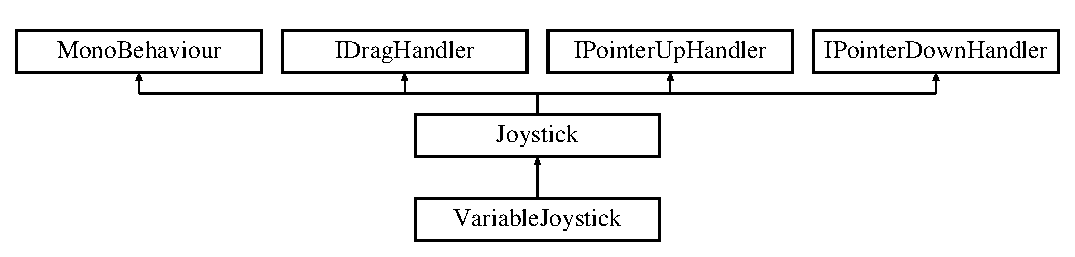
\includegraphics[height=3.000000cm]{class_variable_joystick}
\end{center}
\end{figure}
\subsection*{Public Member Functions}
\begin{DoxyCompactItemize}
\item 
\mbox{\Hypertarget{class_variable_joystick_aeb872ac02d68c91d77faa4438a82eb47}\label{class_variable_joystick_aeb872ac02d68c91d77faa4438a82eb47}} 
void {\bfseries Change\+Fixed} (bool joystick\+Fixed)
\item 
\mbox{\Hypertarget{class_variable_joystick_ae21ea95e4c38d9846a51c1c73813a43a}\label{class_variable_joystick_ae21ea95e4c38d9846a51c1c73813a43a}} 
override void {\bfseries On\+Drag} (Pointer\+Event\+Data event\+Data)
\item 
\mbox{\Hypertarget{class_variable_joystick_acc8ccf667db58a334dbabc60b661dee0}\label{class_variable_joystick_acc8ccf667db58a334dbabc60b661dee0}} 
override void {\bfseries On\+Pointer\+Down} (Pointer\+Event\+Data event\+Data)
\item 
\mbox{\Hypertarget{class_variable_joystick_afa9bf76fbfbffefa6ca1c39badfcb591}\label{class_variable_joystick_afa9bf76fbfbffefa6ca1c39badfcb591}} 
override void {\bfseries On\+Pointer\+Up} (Pointer\+Event\+Data event\+Data)
\end{DoxyCompactItemize}
\subsection*{Public Attributes}
\begin{DoxyCompactItemize}
\item 
\mbox{\Hypertarget{class_variable_joystick_af2091db497b0a0b5a4160f43cafb340e}\label{class_variable_joystick_af2091db497b0a0b5a4160f43cafb340e}} 
bool {\bfseries is\+Fixed} = true
\item 
\mbox{\Hypertarget{class_variable_joystick_a962d78c7313b87cd05d203ba97f4c23d}\label{class_variable_joystick_a962d78c7313b87cd05d203ba97f4c23d}} 
Vector2 {\bfseries fixed\+Screen\+Position}
\end{DoxyCompactItemize}
\subsection*{Additional Inherited Members}


The documentation for this class was generated from the following file\+:\begin{DoxyCompactItemize}
\item 
Iso\+Chai/\+Assets/\+Virtual Joystick Pack/\+Scripts/\+Joysticks/Variable\+Joystick.\+cs\end{DoxyCompactItemize}

%--- End generated contents ---

% Index
\backmatter
\newpage
\phantomsection
\clearemptydoublepage
\addcontentsline{toc}{chapter}{Index}
\printindex

\end{document}
